
% book example for classicthesis.sty
\documentclass[
  % Replace twoside with oneside if you are printing your thesis on a single side
  % of the paper, or for viewing on screen.
  oneside,
  %twoside,
  11pt, a4paper,
  footinclude=true,
  headinclude=true,
  cleardoublepage=empty
]{scrbook}

\usepackage{dissertation}
%---
\usepackage[T1]{fontenc}
\usepackage{textcomp}
\usepackage{float}
%---
\usepackage[titles]{tocloft}
%% Aesthetic spacing redefines that look nicer to me than the defaults.
\setlength{\cftbeforechapskip}{2ex}
\setlength{\cftbeforesecskip}{0.5ex}
%% Use Helvetica-Narrow Bold for Chapter entries
\renewcommand{\cftpartfont}{%
  \fontsize{12}{14}\usefont{OT1}{phv}{bc}{n}\selectfont
}
\renewcommand{\cftchapfont}{%
  \fontsize{11}{13}\usefont{OT1}{phv}{bc}{n}\selectfont
}
\renewcommand{\cftsecfont}{%
  \fontsize{10}{11}\usefont{OT1}{phv}{}{n}\selectfont
}
\renewcommand{\cftsubsecfont}{%
  \fontsize{9}{10}\usefont{OT1}{phv}{}{n}\selectfont
}
\renewcommand{\cftfigfont}{%
  \fontsize{9}{10}\usefont{OT1}{phv}{}{n}\selectfont
}
\renewcommand{\cfttabfont}{%
  \fontsize{9}{10}\usefont{OT1}{phv}{}{n}\selectfont
}
%---
%usepackage[scaled=.92]{helvet}
\usepackage[all]{xy}
\usepackage{circuitikz}

% Title

\titleA{Software Defined Vehicle Networks (SDVN):}
\titleB{Traffic Routing Process Management}
%\titleB{Second line in title (if any)}
%\titleC{Third  line in title (if any)}

% Author

\author{Erikson Neves Tomás}

% Supervisor(es)

\supervisor{Prof. Doutor António Luís Duarte Costa}

\cosupervisor{Prof. Doutor Pedro Nuno Miranda de Sousa}

% Date

\date{\myear} % change to text if date is not today

\makeglossaries  %  either use this ...

\makeindex	% ... or this

\begin{document}\fontfamily{phv}\fontseries{mc}\selectfont
	
% Add acronym definitions
    
% Cover page ---------------------------------------------
%	\thispagestyle{empty}
	%!TEX root = dissertation.tex

\makeatletter

% UM_ENg Logo
\def\UMEng#1#2{\begin{tikzpicture}[
	% bars styling,
	logone/.style={rectangle,fill=white,rounded corners=0.08cm,minimum width=0.16cm,inner sep=0pt},
	bigone/.style={minimum height=0.74cm},
	smaone/.style={minimum height=0.48cm},
	engone/.style={minimum height=0.86cm},
	pos1/.style={xshift=1.3cm,yshift=1.3cm},
	pos2/.style={xshift=3.9cm,yshift=1.3cm}]
	
% Uminho logo
	\fill[fill=#1] (0,0) -- (2.6,0) -- (2.6,2.6) -- (0,2.6) -- cycle;
	\foreach \i in {1,...,3}{
		\node at (\i*120+30:0.45)[logone,bigone,pos1,rotate=\i*120-60]{};
		\node at (\i*120+90:0.60)[logone,smaone,pos1,rotate=\i*120]{};
	}

% EngUminho logo
	\fill[fill=#2] (2.6,0) -- (5.2,0) -- (5.2,2.6) -- (2.6,2.6) -- cycle;
	\foreach \i in {1,...,5}
		\node at (\i*72-90:0.74)[engone,logone,pos2,rotate=\i*72-90]{};
\end{tikzpicture}}

\def\yyy#1{\fontfamily{phv}\fontseries{mc}\selectfont {\ifnum\hide=1\relax\else#1\fi}}
\def\xxx#1{\fontfamily{phv}\fontseries{mc}\selectfont #1}
\def\zzz#1{\fontfamily{phv}\fontseries{mc}\fontseries{b}\selectfont #1}
\def\kkk#1{\fontfamily{phv}\fontseries{mc}\fontseries{b}\selectfont {\ifnum\hide=1\relax\else#1\fi}}

\long\def\coverEtc{
%Logo
~\vskip-4.1cm\rule{4cm}{0pt}\begin{tabular}{l}
\UMEng\umc{eng}
\\\zzz{Universidade do Minho}\rule{0pt}{1cm}
\\\xxx{}{Escola de Engenharia}
\\\xxx{Departamento de  Informática}
\\\rule{0pt}{4cm}
\\\xxx{{\Large\@author}}
\\\rule{0pt}{1em}
\\\zzz{\Large\@titleA}
\\\zzz{\Large\@titleB}
\\\zzz{\Large\@titleC}
\\\rule{0pt}{5cm}
\\\yyy{\large Master dissertation}
\\\yyy{\large Master's in Network Engineering and Telematic Services}
\\\rule{0pt}{6mm}
\\\yyy{\large Dissertation supervised by}
\\\kkk{\@supervisor}\rule{0pt}{4mm}
\\\kkk{\@cosupervisor}
\\\rule{0pt}{4.2cm}
\\\xxx{{\small\@date}}
\end{tabular}
}


\begin{frontcover}
\gdef\umc{um}\gdef\hide{1}
\thispagestyle{empty} \pagecolor{white} \textcolor{black} \coverEtc
\end{frontcover}

\begin{titlepage}
\gdef\umc{um}
\gdef\hide{0}
\thispagestyle{empty} \pagecolor{white}\textcolor{grey} \coverEtc
\end{titlepage}

\makeatother


%rm
	\cleardoublepage
%---------------------------------------------------------
	\pagenumbering{alph}
	\setcounter{page}{0}
%---------------------------------------------------------
% Add acknowledgements

\chapter*{Copyright and Terms of Use for Third Party Work}

This dissertation reports on academic work that can be used by third parties as long as the internationally accepted standards and good practices are respected concerning copyright and related rights.
\vskip 1em
\noindent This work can thereafter be used under the terms established in the license below.
\vskip 1em
\noindent Readers needing authorization conditions not provided for in the indicated licensing should contact the author through the RepositóriUM of the University of Minho.

\section*{License granted to users of this work:}

\CCBY % or replace by one in***************** the list below, cf https://alunos.uminho.pt/PT/estudantes/Formataes/3_Despacho_RT-31_2019_Anexo%203-Informa%c3%a7%c3%a3o-Direitor%20de%20Autor.docx 
%---------
%\CBYNCND
%\CCBYNCSA
%\CCBYNC
%\CCBYND
%\CCBYSA


%---------

\chapter*{Acknowledgements}
Write your acknowledgments here. Do not forget to mention the projects and grants that you have benefited from while doing your research if any. Ask your supervisor about the specific textual format to use. (Funding agencies are quite strict about this.) 

	\cleardoublepage
	
%---------

\chapter*{Statement of Integrity}

I hereby declare that I have conducted this academic work with integrity.
\vskip 1em\noindent
I confirm that I have not used plagiarism or any form of undue use of information or falsification of results along the process leading to its elaboration. 
\vskip 1em\noindent
I further declare that I have fully acknowledged the Code of Ethical Conduct of the University of Minho.
	
%---------

% Uncomment as wished
	
% Add abstracts (en,pt) -----------------------------------------------------------
\chapter*{Abstract}
	The Vehicular Ad hoc Networks (VANETs) were created by applying the principles of MANETs networks, i.e. the spontaneous creation of a wireless network of mobile devices, in this case vehicles that exchange relevant information with each other. In this sense, vehicle-to-vehicle and vehicle-to-road/infrastructure communication architectures may coexist in VANETs in order to provide road safety, navigation instructions and other relevant services in this context. VANETs are a fundamental part of the intelligent transport systems (ITS) framework.
    On the other hand, the emergence of the recent concept of Software-Defined Networking (SDN), through the separation of the control and data plane and a centralized view of the network, has brought greater flexibility in the management and configuration of network infrastructures, opening also the possibility of developing innovative and smarter mechanisms in the area of communication networks. Thus, several studies defend the relevance of joining these two areas, in the area called Software Defined Vehicular Networks (SDVN), where one or more SDN controllers interact and control all or part of the underlying vehicular network.

\paragraph{Keywords:} SDN (software defined Network), OpenFlow, Mininet-wifi, Ryu, Vanets, SUMO.

	\cleardoublepage

\chapter*{Resumo}
As Redes Ad hoc Veiculares (VANETs) foram criadas aplicando os princípios das redes MANETs, ou seja, a criação espontânea de uma rede sem fio de dispositivos móveis, neste caso veículos que trocam informações relevantes entre si. Nesse sentido, arquiteturas de comunicação veículo-veículo e veículo-estrada/infraestrutura podem coexistir em VANETs para fornecer segurança rodoviária, instruções de navegação e outros serviços relevantes neste contexto. As VANETs são uma parte fundamental da estrutura dos sistemas de transporte inteligentes (ITS).
Por outro lado, o surgimento do recente conceito de Software-Defined Networking (SDN), através da separação do plano de controle e dados e uma visão centralizada da rede, trouxe maior flexibilidade na gestão e configuração das infraestruturas de rede, abrindo também a possibilidade de desenvolver mecanismos inovadores e mais inteligentes na área das redes de comunicação. Assim, vários estudos defendem a relevância da junção destas duas áreas, na área denominada Software Defined Vehicular Networks (SDVN), onde um ou mais controladores SDN interagem e controlam toda ou parte da rede veicular subjacente. 

\paragraph{Palavras-chave:} SDN (Software-Defined Network), OpenFlow, Mininet-Wifi, Ryu Controller, Vanets, SUMO.


	\cleardoublepage
	
	\pagenumbering{roman}
	\setcounter{page}{3}
	%pagestyle{fancy}   % -------- removed
	%rm
	
	% Document
	\cleardoublepage
    \phantomsection
    \addcontentsline{toc}{chapter}{Contents}
	\tableofcontents
	
	\cleardoublepage
	\listoffigures
	
	\cleardoublepage
	\listoftables
	
	\cleardoublepage
	\lstlistoflistings
	
	% Add list of acronyms
	\cleardoublepage
	\pagenumbering{arabic}
	\setcounter{page}{3}


\part{Introduction}
\chapter{Introduction}
	%Context, motivation, main aims	
	
\section{Motivation}

The main motivation behind this work is to introduce the network virtualization in a VANET environment leveraged by SDN technology.
\par{Vehicular Ad hoc Networks (VANETs) were created by applying the principles of MANETs networks, i.e. the spontaneous creation of a wireless network of mobile devices, in this case vehicles that exchange relevant information with each other. In this sense, vehicle-to-vehicle and vehicle-to-road/infrastructure communication architectures may coexist in VANETs in order to provide road safety, navigation instructions and other relevant services in this context. VANETs are a fundamental part of the intelligent transport systems (ITS) framework.}
\par{
On the other hand, the emergence of the recent concept of Software-Defined Networking (SDN), through the separation of the control and data plane and a centralized view of the network, has brought greater flexibility in the management and configuration of network infrastructures, opening up the possibility of developing innovative and smarter mechanisms in the area of communication networks. Thus, several studies defend the relevance of joining these two areas, in the area called Software Defined Vehicular Networks (SDVN), where one or more SDN controllers interact and control all or part of the underlying vehicular network.}
\par{
In this context, we intend to propose and develop in this project a demonstrative prototype of a management system for traffic routing processes in vehicular networks. This system must operate under the command of a controlling entity (eg the SDN controller) that will establish the specific rules for routing traffic for communications carried out between the elements of the vehicular network and/or between these and the entities or systems residing in the network infrastructure support to the vehicular network. The specified rules may depend on the specific case study, the application considered, the type of traffic being considered, or other parameters that are deemed relevant. The project should consider a simulation environment constituted by the Mininet-Wifi simulator, which includes the implementation of the protocol stack for vehicular networks, together with the SUMO urban mobility simulator, making therefore its practical exploration crucial  and the analysis of its possible integration form. with components of SDN architectures.}

\section{Objectives}
\label{objectives}
\par{This dissertation intends to evaluate the possibility of integrating the Software Defined Networks and Vehicular Networks, specifically in the management of routing processes. The objective is to create a simulated prototype that concretely demonstrates this possibility, allowing an assessment of its practical usefulness and eventual added value compared to other alternatives.}

To achieve the project objectives the following tasks are defined:
i) Initial investigation on VANETS, SDN and SDVN topics;
ii) Familiarization and operation of the Mininet-Wifi + SUMO simulator and the ability to integrate it with the SDNs area;
iii) Specification of an illustrative system for managing traffic routing processes in the vehicular network through SDNs;
iv) Implementation of a prototype of the proposed system;
v) Definition of the appropriate test scenario(s);
vi) Illustrative tests of the solution's operation.
The analysis of the results obtained will allow concluding on the suitability of the solution.

\section{Dissertation structure}
This dissertation is composed of 5 chapters:
\begin{itemize}
\item Chapter 1
\par {The first chapter presents the reasons that led to the completion of the dissertation, introducing the current problem, the motivation, and the proposed objectives for its resolution.}
\item Chapter 2
\par{Then, in the second chapter, the current state of the art is demonstrated. A background is made on the main topics and the tools that made it possible to carry out the project are described, such as the tools that currently exist in order to try to solve the presented problems.}
\item Chapter 3
\par{In the third chapter, we have the core of the dissertation, the tasks defined to achieve the proposed objectives. Its operation, problems encountered in its elaboration and the respective solutions are described in this chapter.}
\item Chapter 4
\par{In the fourth chapter there is information corresponding to the simulations. This chapter describes the environment where these were carried out, their results and their analysis, taking into account the proposed objective for the project.}
\item Chapter 5
\par{The fifth chapter is the last of the dissertation. Here, the final survey of the results achieved during its elaboration is carried out. Possibilities of continuing the development of the project in future works are also mentioned.}
\end{itemize}


\chapter{State of the art}
\label{State of-the art}
At a glance, this portion of the report   provides the main concepts involved in this thesis, inserting firstly the key points of Software Defined Network (section \ref{Software-Defined Network}), that consists of separating the control functions from the forwarding functions which enables a greater automation and programming in the network. The next concept being introduced is the  concept of Ad hoc vehicular networks (Vanets) as a specialisation of Ad hoc mobile networks (Manets), applied to vehicles such as cars, trains and buses. These networks are implemented over a layer of wireless communication, such as Bluetooth, Wi-Fi, 4G or even 5G (section \ref{Vehicular Ad hoc Networks}).  With the advancement of the Vanets, a new networking paradigm  called software-defined vehicular networks (SDVN) (section \ref{Software-Defined Vehicular Networks}) is borned, The basic idea of it, is to introduce the network virtualisation in a Vanet environment boosted by the SDN technology. Still in the context of Vanets, the concept of SUMO (subsection \ref{SUMO}) is also discussed. SUMO is a highly portable, microscopic and continuous open source urban mobility package designed to handle large networks. It allows an intermodal simulation including pedestrians and it comes with a large set of tools for creating diverse scenarios. Sequently the concept of Mininet-Wifi (subsection \ref{Mininet-Wifi}) is addressed, which is an extension of the Mininet (SDN emulator), that enlarges the features contained in Mininet by adding Wifi stations and virtualised access points based on standard Linux wireless drivers and the 80211-hwsim wireless simulation driver. 
 At last the concept of SDN Controllers is emphasised as the one that will allow the control of our scenario. Among the many SDN Controllers, the Ryu Framework (subsection \ref{Ryu-Controller}) was chosen as the one to work with.The Ryu SDN Framework is an SDN controller written in python that provides the libraries needed to develop SDN applications.Its structure eases the development by providing the basic functions to control the data plan and the functions for SDN applications.

\section{Software-Defined Network}
\label{Software-Defined Network}

%This section provides a description of the SDN and describesuilt to achieve network requirements.\par
Software-Defined Networking (SDN) is an emerging dynamic, manageable, economical, and adaptable architecture, These features make it a ideal for the dynamic, high-bandwidth nature of today’s applications. This architecture aims to decouple network control and routing functions, allowing the network control to become directly programmable and the underlying infrastructure to be abstracted for network applications and services.

\subsection{Software-Defined Network Architecture}
\label{Software-Defined Network Architecture}

The Software-Defined Network Architecture is:

\begin{itemize}
    \item Directly Programmable\par
Network control is programmable directly because it is decoupled from routing functions.
    \item Agile \par
Abstracting routing control allows administrators to dynamically adjust the flow of the traffic across the network to meet the changing needs.
    \item Centrally Managed\par
Network intelligence is (logically) centralized on software-based SDN controllers that maintain a global view of the network, which appears as single logical switch to the applications and  policy mechanisms.
    \item Programmatically Configured \par
SDN allows network managers to configure, manage, secure, and optimize the network resources very quickly through automated, dynamic SDN programs, which they themselves can write because the programs do not rely on proprietary software.
    \item   Based on Open and Vendor-Neutral Standards \par
When implemented through open standards, thr SDN simplifies the design and the operation of the network because the instructions are provided by SDN controllers instead of multiple vendor-specific devices and protocols.
\end{itemize}

As shown in Figure \ref{SDN-architecture}, the SDN architecture is divided into three plans, namely: data plan, control plan and management plan. The Data Plan is made up of the network infrastructure and the Southbound Interface. The middle plan, called the control plan, is made up of three layers: the network Hypervisor, the network controller(s) and the Northbound Interface. Finally, the top layer, called the management plan, is structured in three layers: the languages and approaches used in virtualization, the programming languages and the network applications. 

\begin{figure}[H]
\begin{center}
	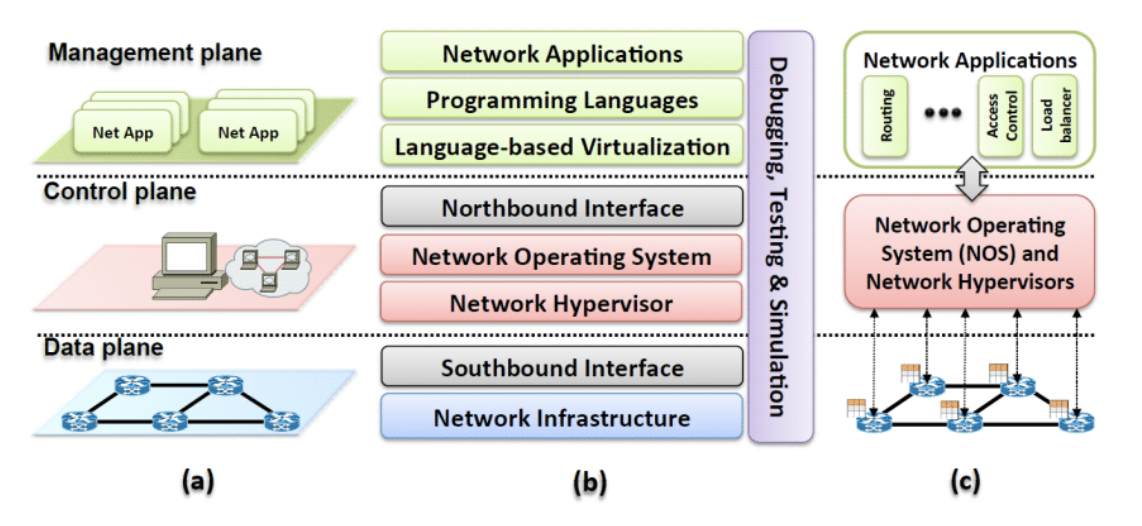
\includegraphics[width=1\textwidth]{img/arquitetura geral.png}
\end{center}
\caption{SDN architecture divided into a) plans b) layers and c) design
of architecture ~\cite{primeiro}}
\centering
\label{SDN-architecture}
\end{figure}

Conventional IP networks have major limitations, as the internet was not designed taking into account the use we give today. Contrary to what happens in conventional IP networks (Figure \ref{The modern approach to computing and networking})  where the functionalities are decentralized, the SDN appears to solve the problems we face. SDN is centralized to provide connection network domains between the control and data plans on the same infrastructure. Nevertheless, SDN allows backward compatibility with several existing protocols and standards (IP, ARP, VLAN, Ethernet, etc.) ~\cite{primeiro}.\par

\begin{figure}[H]
\begin{center}
    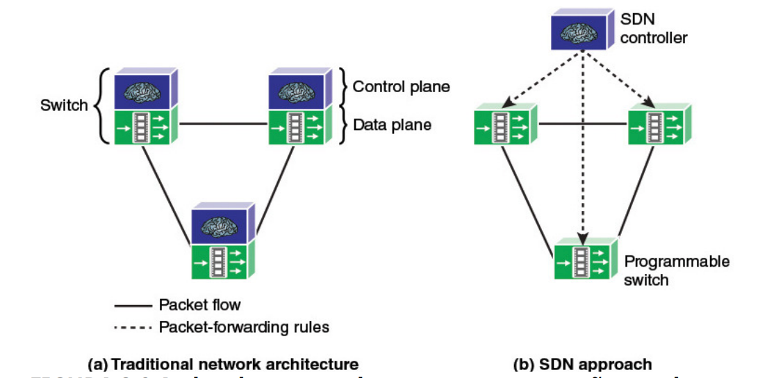
\includegraphics[width=1\textwidth]{img/sdna.png}
\end{center}
  \caption{The modern approach to computing and networking ~\cite{stallings2015foundations}}
\centering
\label{The modern approach to computing and networking}
\end{figure}


The core architecture of SDN is divided into three layers as illustrated in the figure below (Figure \ref{Software-defined networking a generic architecture}).\par


\begin{itemize}
    \item 
    Application layer: An application layer is made up of applications that communicate securely with the control layer controller through interfaces, called Northbound APIs. The most commonly used API is the REST API (Download State Representation) to provide Northbound APIs. Applications on SDN can be like Firewall, load balancer, etc.
    
    The upper layer (application layer) is the layer responsible for defining rules and offers several services, including quality of service, firewall, routing, access control, IDS/IPS, proxy service, and monitoring balancer.\par
    
    \item
    
    The middle layer, called the control plan, is an abstraction of the network topology . The controller is the main component responsible for establishing flow tables and policies for data processing, in turn also abstracts network complexity and network information through the Southbound API. It is also responsible for keeping  a holistic view of the network up-to-date.The Southbound API communications can be deployed in two different scenarios:

\begin{itemize}
    \item 
    In-band communication: in this scenario, the traffic between the controller and any network device must obey the dictated flow rules. \par
    \item Out-of-band communication: here, the traffic does not follow the flow rules.This type of communication requires VLAN implementation to isolate the traffic flow from communications, which depends on the OpenFlow rules. There are also east/west APIs (eg HyperFlow) ~\cite{hyperflow} where multiple controllers exchange control information about the flow in the data plan. There are many controllers written in different programming languages (Python, C/C++, Java, Ruby, etc.) and platforms like NOX, Flood-light, Beacon, Maestro and Trema.
\end{itemize}

    \item
    Physical layer or Infrastruture layer: this layer which is also known as the data plan, provides network devices such as physical/virtual switches, routers and access points. Switches just perform the actions as per the controller. One interface that they use to communicate with a control layer is the Southbound APIs. The OpenFlow protocol is the most common protocol used to provide Southbound API.
    This layer is responsible for all the data activities including forwarding, fragmentation and reassembly. 
This architecture will be further explored in the following sections.\par
\end{itemize}

\begin{figure}[H]
\begin{center}
  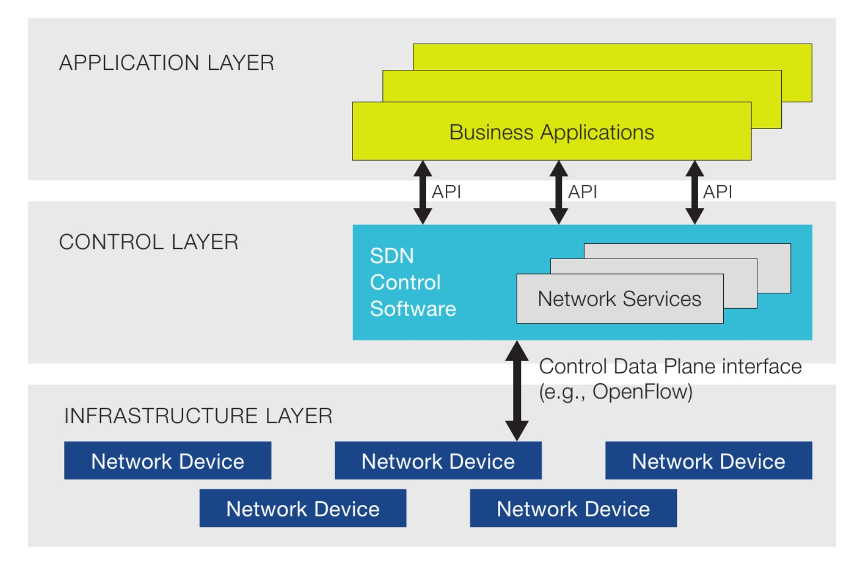
\includegraphics[width=0.70\textwidth]{img/archi.png}
\end{center}
  \caption{Software-defined networking a generic architecture}\par
  {From: https://learning.knetsolutions.in/docs/ryu/#2-sdn-overview}
  \centering
\label{Software-defined networking a generic architecture}
\end{figure}

\subsection{Open-Flow }
\label{Open-Flow}
OpenFlow establishes the communication between the control plan and the data plan. It implements one of the first standards in SDN, making it possible for the SDN controller to interact directly with the forwarding nodes – switches and routers – in a network ~\cite{openflowintro}.\par
In a simpler way, OpenFlow in the SDN framework it consists of an OpenFlow controller and several OpenFlow switches that the controller is associated with to perform actions. briefly, when a user packet arrives at an OpenFlow switch, it is checked against an entry in a flow table to see if it matches; if this happens, the packet will be processed and forwarded according to the specified actions, sometimes visiting additional flow tables as specified by the actions. If the packet does not match the last flow table entry, the packet is dropped if there is no missing table entry.


\subsubsection{Data plan}.

OpenFlow is a logical data plan functionality framework and protocol between the SDN driver and the network devices.
In an SDN architecture the infrastructure represents a set of equipment, called forwarding devices, which can be in switches, routers and/ or middleboxes. Different from the  traditional built-in devices with control system
allowing them to take decisions independently, these only proceed to packet forwarding. An Openflow protocol-enabled routing device consists of one or more flow tables, an Openflow channel with connection to the controller (from the control plane) and a protocol (Openflow protocol) that allows the controller to add, update or remove flow inputs. A flow table of an Openflow forwarding device consists of a set of inputs, each consisting of three fields, namely a match field defined by a set of information (see Figure \ref{const-flow-entry}) a field with the action associated with the package and a counter used for statistics.
The matching process is started in the first table and can continue through the following tables. If there is no entry matching the package to be treated, it can be discarded and  forwarded to the controller or sent to the following table.
This process repeats until the package goes through the last table.
That is, when there is package matching with a table entry, the package can be 1) routed to a particular output network interface, 2) encapsulated and forwarded to the controller, 3) discarded or 4) shipped to the next flow table through the pipeline process. 

\begin{figure}[H]
\begin{center}
  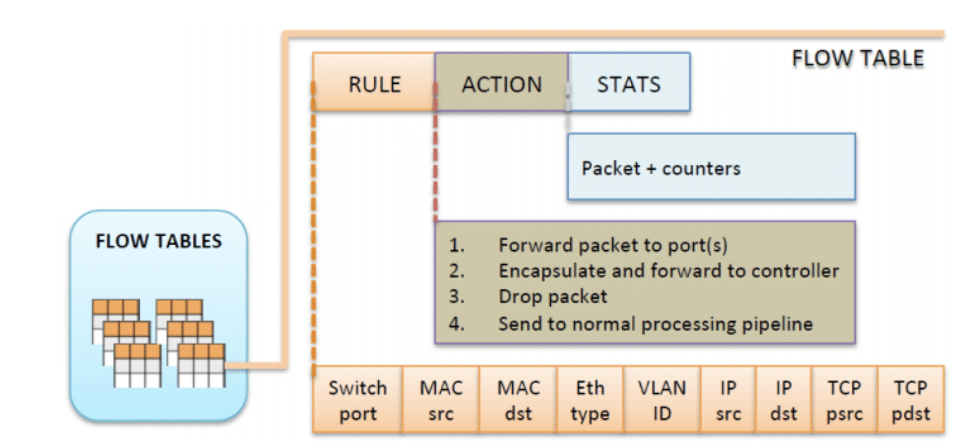
\includegraphics[width=0.70\textwidth]{img/flow table.png}
\end{center}
  \caption{Constitution of flow entries ~\cite{primeiro}}
  \centering
\label{const-flow-entry}
\end{figure}


\subsubsection{Control Plan}\par


%Terminamos here 
%As we can see on Figure \ref{Figure-Northbound}
%As we can see on subsection\ref{section-SDN}


%\section{Citations}
%Example of a citation: \cite{GRM97}, cf.\ this entry in the \Bibtex\ file.
%Another way of citing is \citep{KeR88}


Data Plan Functions

The functions carried out by network data plan devices also called network elements or data plan switches are shown in Figure \ref{Data Plane Network Device}. The main functions of the network device are as follows:

\begin{figure}[H]
\begin{center}
  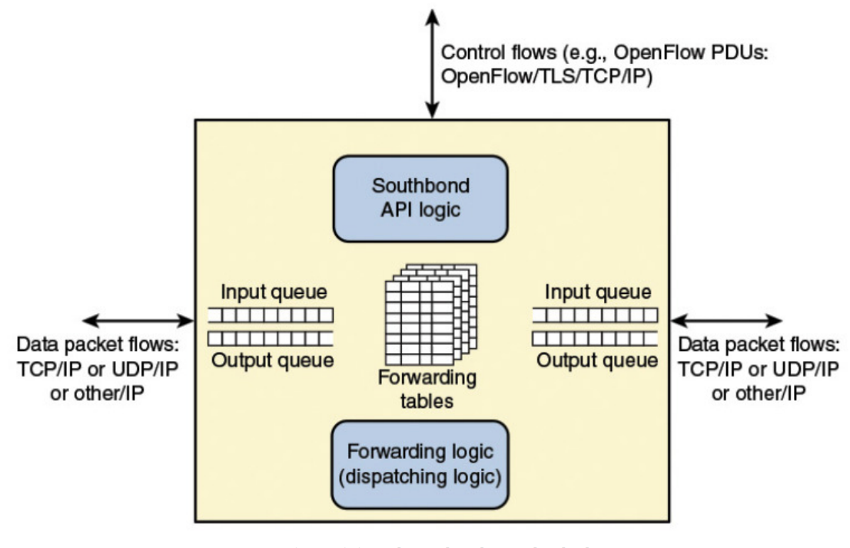
\includegraphics[width=0.75\textwidth]{img/enc.png}
\end{center}
  \caption{Data Plan Network Device ~\cite{stallings2015foundations}}
  \centering
\label{Data Plane Network Device}
\end{figure}


Control Support Function: It interacts and allows programming through resource control interfaces with the SDN control layer. The OpenFlow switch communicates with the controller, which is managed by the controller through the OpenFlow switch protocol.\par

Data Forwarding Function: it accepts incoming data streams from other network, end devices and forwards them with calculated and established data forwarding paths according to the rules defined in SDN applications.\par

The network device forwarding rules are incorporated in the forwarding tables which show certain categories of packets what the next hop in the route should be for. The network device may change the packet header before forwarding or discard the packet, in addition to the simple forwarding of packets. As illustrated, incoming packets can be placed in the input queue awaiting processing by the network device, and forwarded packets are normally placed in an output queue, waiting for transmission.\par
In Figure \ref{Data Plane Network Device}, the network device shows three I / O ports: one for SDN-controller control communication, and two for data packet input and output. The network device could have more than two I/O ports for packet flows in and out of the device for multiple SDN controllers ~\cite{stallings2015foundations}.\par

Data Plan Protocols

Figure \ref{Data Plane Network Device} indicates the protocols supported by means of the network device. Data packet flows encompass streams of IP packets. It may be vital for the forwarding table to outline entries based totally on fields in upper-level protocol headers, along with TCP, UDP or some other protocol. The IP header examines by the network device and likely different headers in every packet and makes a forwarding decision. The other important data traffic flow is via the southbound application programming interface (API), consisting of OpenFlow Protocol Data Unit (PDUs) or a few similar Southbound API protocol traffic ~\cite{stallings2015foundations}.\par

\subsection{OpenFlow Logical Network Device}

The distinguishing properties of SDN must be evaluated. The two key aspects of the SDN are a common logical architecture on SDN devices and an SDN controller protocol with network devices.
That means that the common logical architecture is required for all switches, routers, and other network devices to manage with an SDN controller. The SDN unification feature allows various providers to implement this logical architecture in various ways to construct network devices that operate under a SDN controller with a uniform logical switching function.
The SDN controller and the network device require a standard and a secure protocol.
The first software-defined networking (SDN) interface is OpenFlow (OF). The SDN Controller initially identified a networking protocol that enables it to deal directly with the forwarding plan of both physical and virtual network equipment, such as switches and routers, to best suit evolving business needs. OpenFlow is specified by the Open Networking Foundation (ONF) OpenFlow Switch Specifications ~\cite{stallings2015foundations}.

The key elements of an OpenFlow environment consisting of SDN controllers, including OpenFlow software, OpenFlow switches and end systems, are described in Figure \ref{OpenFlow Switch Context}.\par

\begin{figure}[H]
\begin{center}
  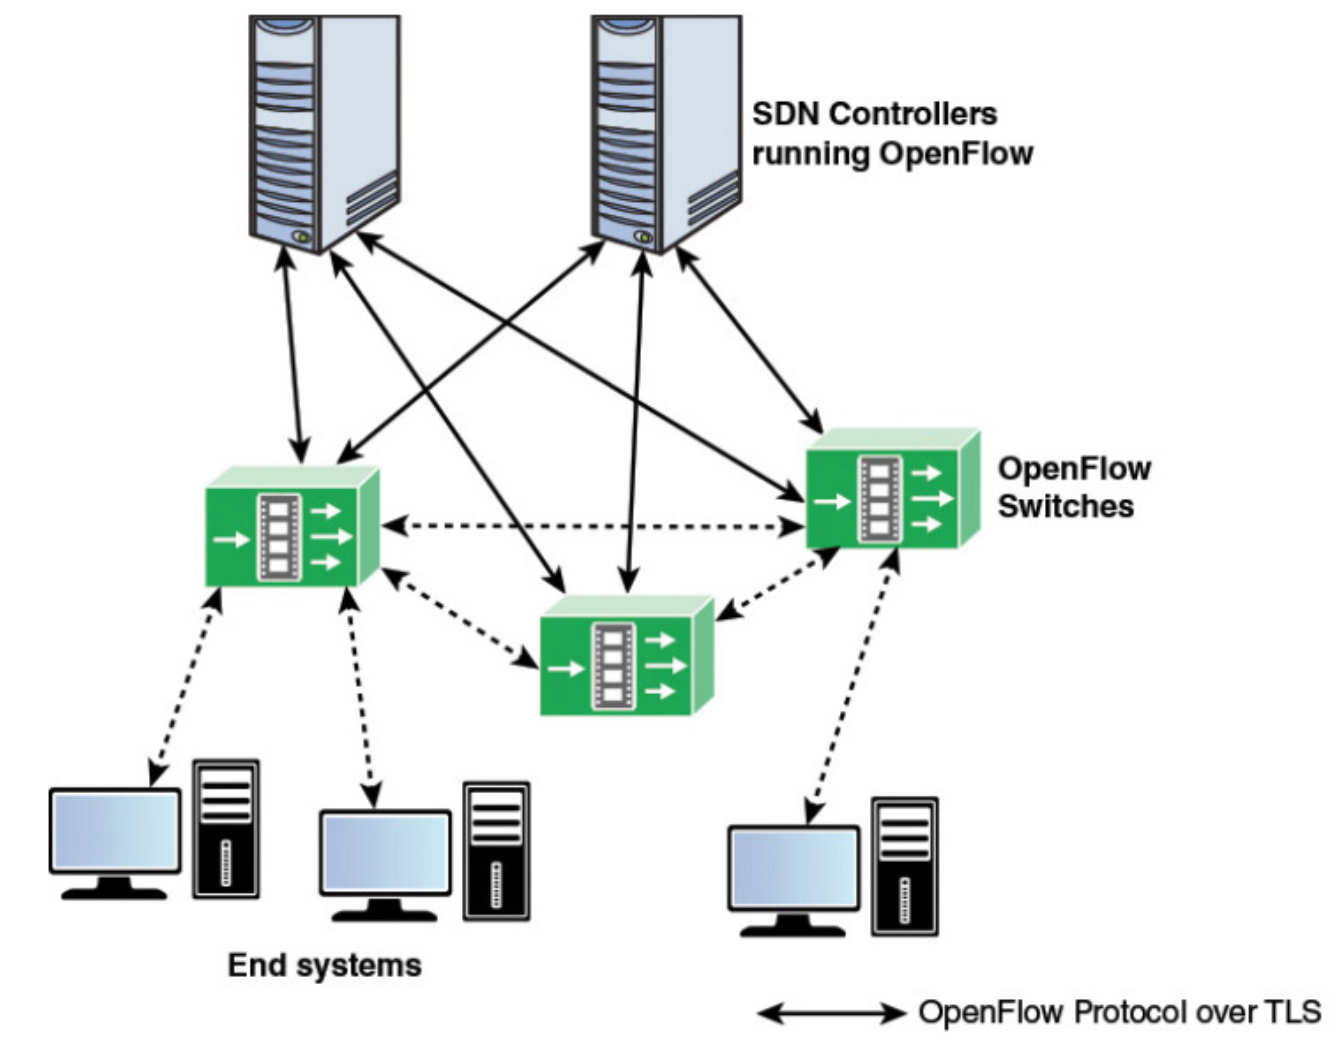
\includegraphics[width=0.6\textwidth]{img/switchdev.png}
\end{center}
  \caption{OpenFlow Switch Context ~\cite{stallings2015foundations}}
  \centering  
\label{OpenFlow Switch Context}
\end{figure}


Figure \ref{OpenFlow Switch} displays the main OpenFlow switch components. The communication standard used by SDN, known as OpenFlow, and developed by the Open Network Foundation, does the implementation of the Transport Layer Security (TLS). Each switch connects to the other OpenFlow switches and, probably, to the consumer devices used for packet flows of the sources and destinations. The Switch contains an interface called OpenFlow channel .Open Flow ports are used for interfaces. The transfer to the SDN controller is also attached to the OpenFlow port.\par

\begin{figure}[H]
\begin{center}
  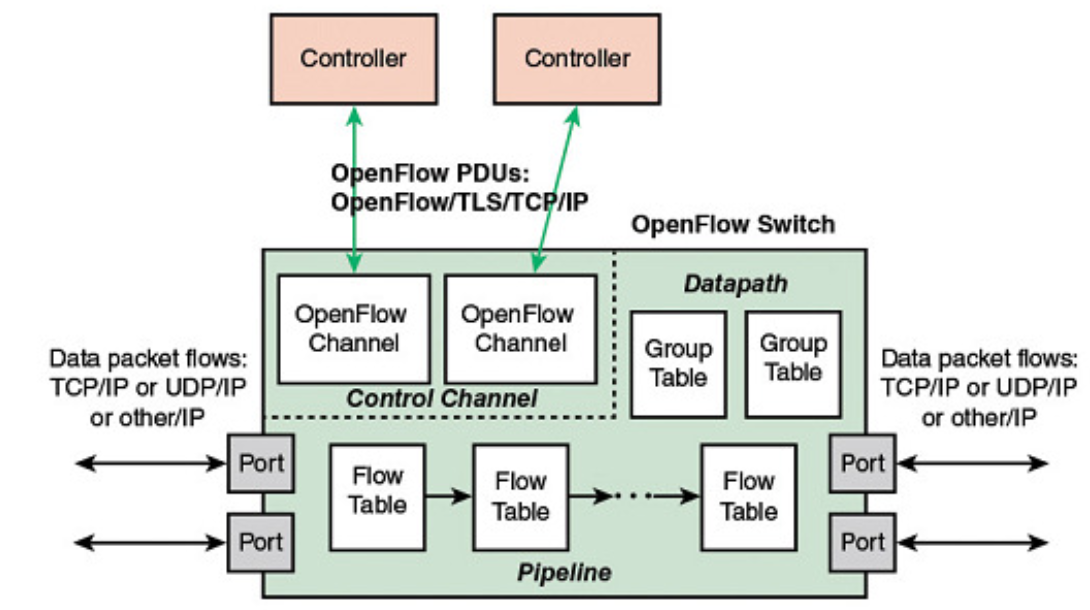
\includegraphics[width=0.8\textwidth]{img/porswit.png}
\end{center}
  \caption{OpenFlow Switch ~\cite{stallings2015foundations}}
  \centering  
\label{OpenFlow Switch}
\end{figure}


Three ports are specified by OpenFlow: Physical ports:
   The physical ports in OpenFlow are the ports which have been connected to a switch’s hardware interface. For instance, physical ports map the Ethernet interfaces one-to-one on an Ethernet switch.\par

   Logical port: The logical ports for OpenFlow are switched ports that do not meet the hardware of the switch directly. Logical ports are higher level abstracts which can be specified through non-OpenFlow methods (e.g. link aggregation classes, tunnels, loopback interfaces) in a switch. 
   Logical ports will encapsulate packets and map them through many physical ports. The processing through the logical port will be transparent to the OpenFlow processing, and ports such as OpenFlow physical ports can communicate with OpenFlow processing.
   
   Reserved Ports: This specification defines the OpenFlow reserved ports. They signify the  basic forwarding actions, such as sending to the controller, flooding or transportation, utilizing non-OpenFlow methods, such as "normal" switch processing. 
   A series of tables are used within each switch to control the packet flows via the switch. 
   In the logical switch framework the specification OpenFlow describes three types of tables. A flow table corresponds to the incoming packets in one flow and describes the functions on the packets. Multiple flow tables can be used in a pipeline fashion. A flow table may direct a flow relate to a group table that can cause a variety of actions involving one or more flows. A meter table may cause multiple actions related to the performance on a flow. The controller will add, update and delete tables of flow entries both responsively and constructively utilizing the OpenFlow switch protocol.\par

\subsubsection{Flow Table Structure}

The flow table represents the fundamental aspect of the logical switch architecture. Each packet entering a switch is loaded with one of the flow tables. A number of rows are specified in the following table, each of which consists of 7 elements, known as entries (see Figure \ref{OpenFlow-Table-Entry-Formats} ).

\begin{figure}[H]
\begin{center}
  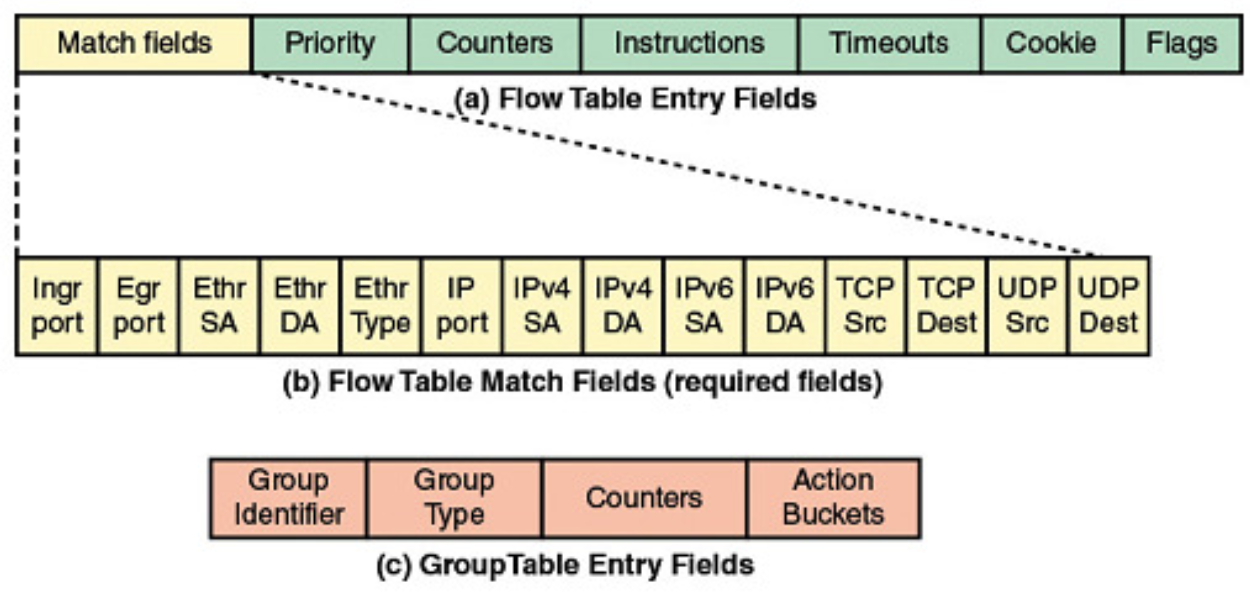
\includegraphics[width=0.8\textwidth]{img/grtable.png}
\end{center}
  \caption{OpenFlow Table Entry Formats ~\cite{stallings2015foundations}}
  \centering  
\label{OpenFlow-Table-Entry-Formats}
\end{figure}


A flow table consists of flow entries.

\begin{itemize}
    \item 
    match fields: To match the packets. Which comprise the ingress port, the packet headers, and the metadata listed in a previous table optionally.
    \item
    Priority: matching precedence of the flow entry.
    \item
    counters: updated when the packets are matched.
    \item
    instructions: to modify the action set or pipeline processing.
    \item
    timeouts: maximum amount of time or idle time before flow is expired by the switch.
    \item
    cookie: opaque data value chosen by the controller. May be used by the controller to filter flow statistics, flow modification and flow deletion. Not used when processing packets.
    
    \item
    Flags: Flags modify the handling of flow entries; for instance the flag OFPFFSENDFLOWREM causes messages removed from flow entry.
\end{itemize}



\section{Vehicular Ad hoc Networks}
\label{Vehicular Ad hoc Networks}

Over the past ten years, Vehicular Ad Hoc Networks (VANETs) have received significant attention from the academic and the industrial communities. A VANET is a particular class of Mobile Ad Hoc Network (MANET) in which mobile nodes are vehicles. VANETs are characterized by: 1) high, geographically restricted and predictable node mobility due to the route layout; 2) a rapidly changing network topology; and 3) a highly unstable communication environment . In VANETs, we can identify four types of communication patterns, as illustrated in Figure \ref{Types-of-communication patterns-on-VANETs}: Vehicle to Vehicle (V2V), Vehicle to Infrastructure (V2I), Vehicle to Pedestrian (V2P) and Vehicle to Network (V2N). Typically, Vehicle To Everything (V2X) is used to refer to the four types of communication ~\cite{vanets}.

\begin{figure}[H]
\begin{center}
  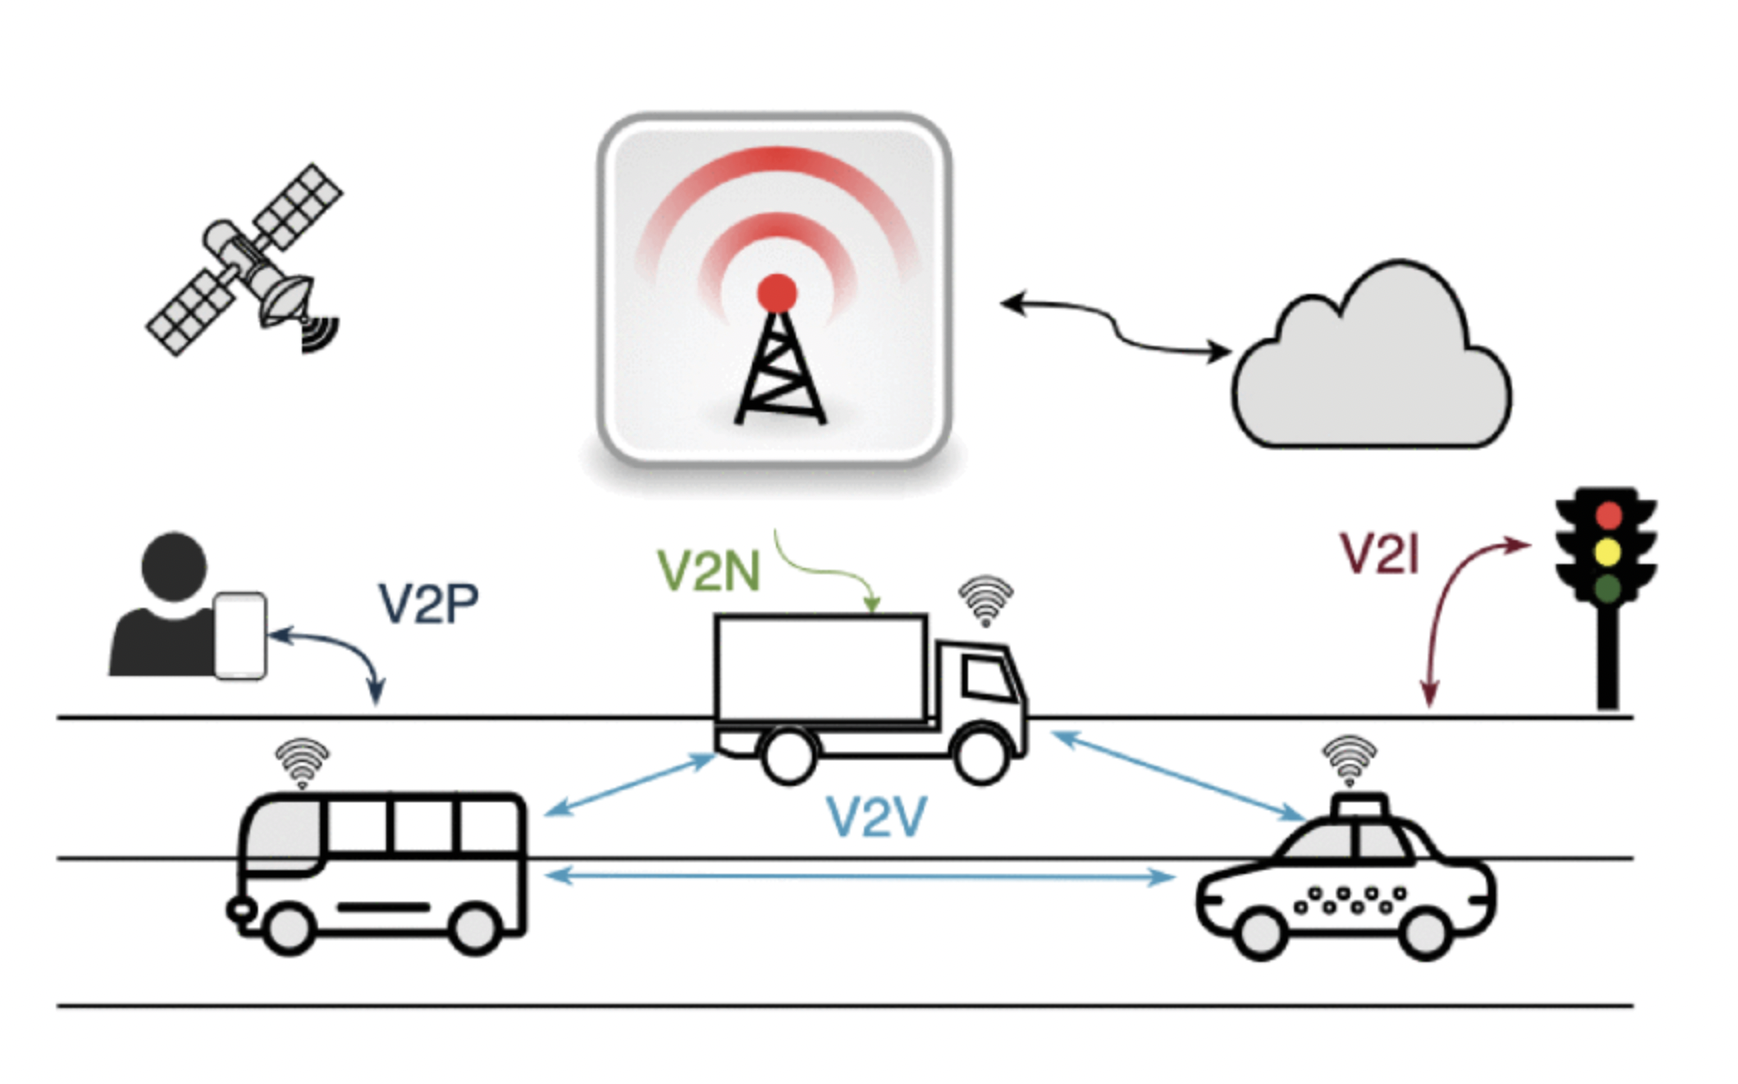
\includegraphics[width=0.8\textwidth]{img/types vanets.png}
\end{center}
  \caption{Types of communication patterns on VANETs ~\cite{vanets}}
  \centering  
\label{Types-of-communication patterns-on-VANETs}
\end{figure}

Vehicular Ad Hoc Network (VANET) utilizes cars as a mobile node to create a mobile network. Vehicles act as a mobile node with the corresponding network. The basic aim of VANET is to improve and increase the safety on our roads and road users, the comfort of passengers, and also aid the communication between vehicles and roadside equipment. The VANET communication medium is installed on each node (vehicle). As shown in Figure \ref{Vanets-Best}, each vehicle has its own communication wireless network card which allows ease of communication flow between vehicles and roadside units. \par

\begin{figure}[H]
\begin{center}
  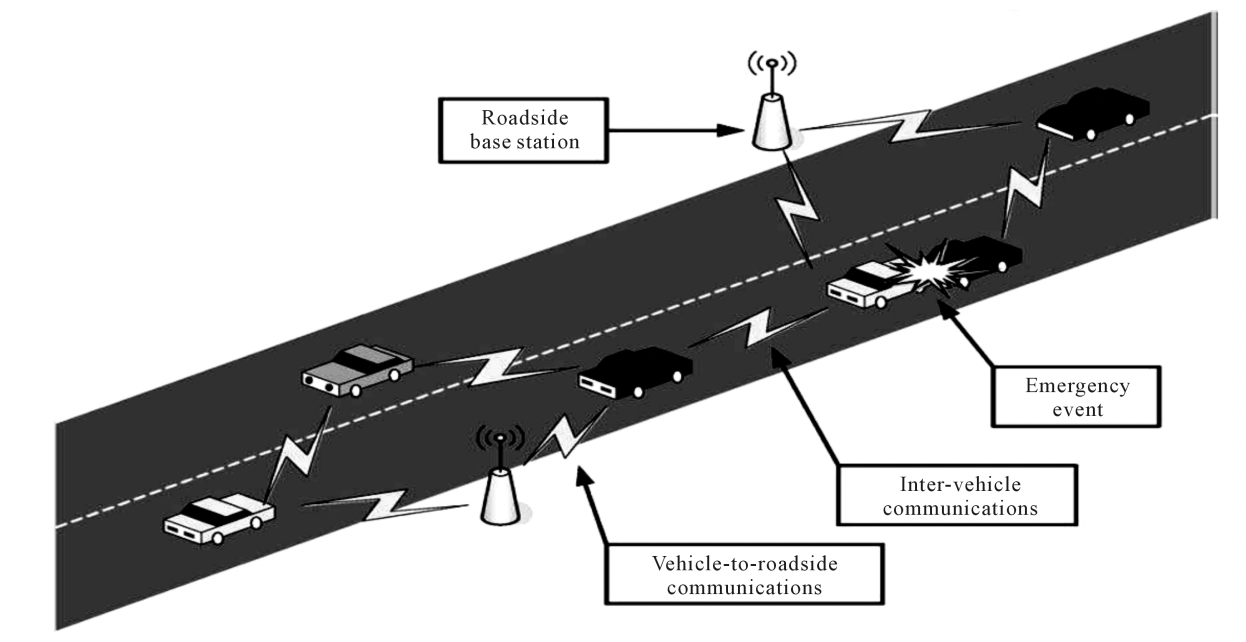
\includegraphics[width=0.8\textwidth]{img/v1.png}
\end{center}
  \caption{A VANET consists of vehicles and roadside base stations that exchange primarily safety messages to give the
drivers the time to react to life-endangering events. ~\cite{vanetusarlater}}
  \centering  
\label{Vanets-Best}
\end{figure}


Figure \ref{Vanets-Best-b} Shows the different domains that exist in VANET. The Mobile Domain consists of (Vehicle and Mobile Devices) such as PDA, Smart Phones, and Laptop etc. The Generic Domain consists of (Internet Infrastructure and Private Infrastructure) such as nodes and servers. While the Infrastructure Domain consists of (Road Infrastructure or Units and the Central Infrastructure) such as the RSU that communicate with the vehicle along the road, and the management center that communicates with the internet ~\cite{vanetusarlater}.\par
The Mobile Domain communicates with the Infrastructure Domain and the Infrastructure Domain communicates with the Generic Domain and data flows between the different domain to provide effective and efficient use of the road by the road users.\par
Since the communication is provided in 2 different way in VANET,  here are some fixed node that act as a roadside unit or equipment which enables the ease of VANET to serve as a gateway to the internet and also in accessing geographical data. Each node in the VANET doesn’t only participate in data transmission and receiving, they also act as a wireless router of the network as different nodes communicate via their own communication range, permitting cars in the region of 100 to 300 meters of each other to join the network, and create a network with a wide range. As cars fall out of the signal range and drop out of the network, other cars can join in, connecting vehicles to one another so that a mobile Internet is created ~\cite{vanetusarlater}.


\begin{figure}[H]
\begin{center}
  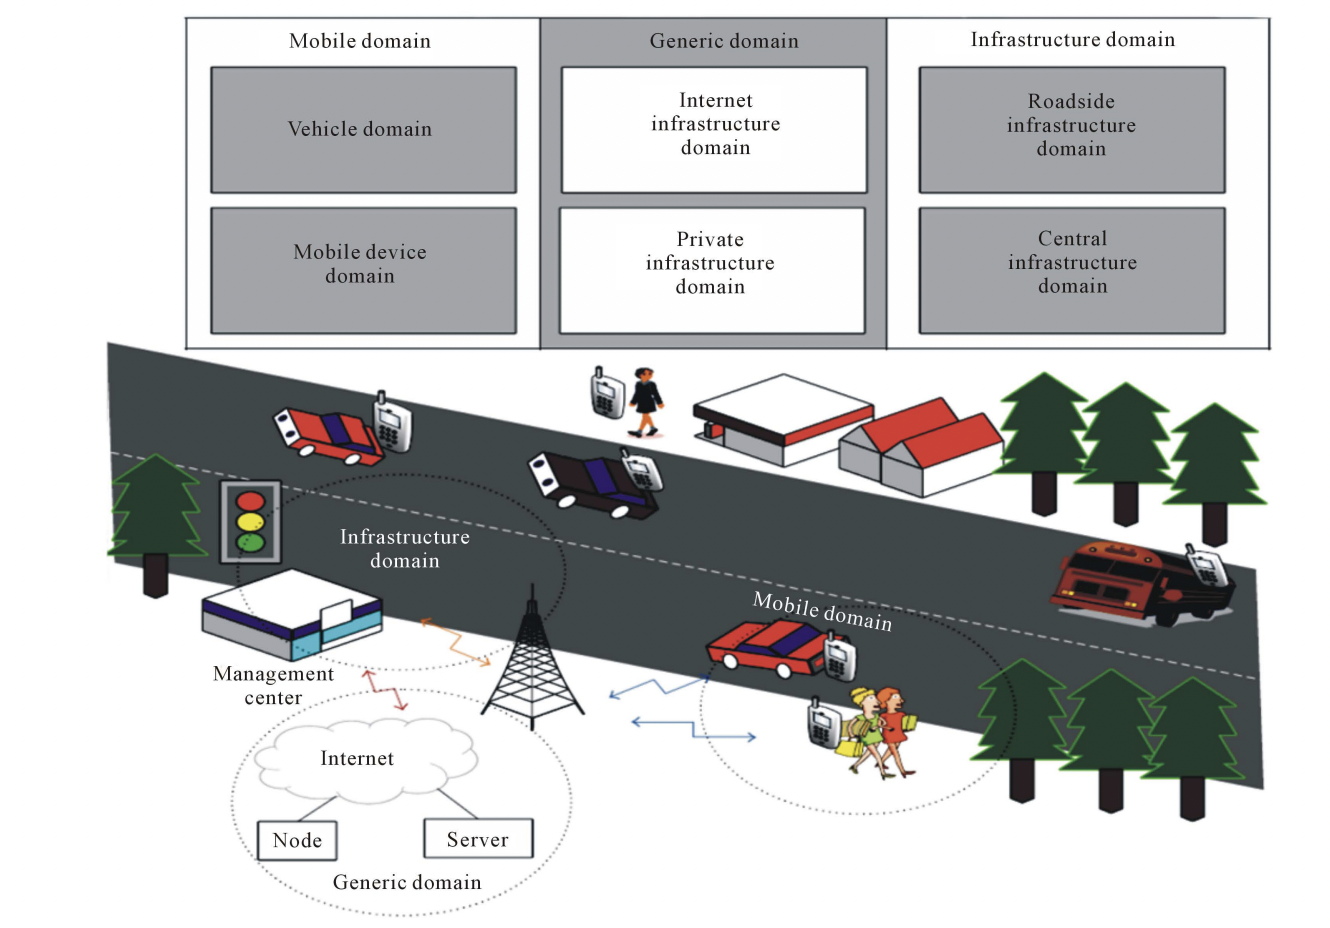
\includegraphics[width=0.9\textwidth]{img/v2.png}
\end{center}
  \caption{VANET system sphere. ~\cite{vanetusarlater}}
  \centering  
\label{Vanets-Best-b}
\end{figure}




\subsection{Generic VANET Architecture}


The two main communication models in VANETs are classified as Vehicle-to-Vehicle (V2V) communication and Vehicle to Infrastructure (V2I). V2V communication is the ability of exchanged transmission between different vehicles while V2I is the communication between the vehicles and the road-side framework. The main communication module consists of Road-Side Unit (RSU), on-board unit (OBU), and trusted authority (TA) as shown in Figure \ref{VANETs architectures}. The RSU unit is fixed and made up of a transceiver that sends and receives information from the OBU and TA.


\begin{figure}[H]
\begin{center}
  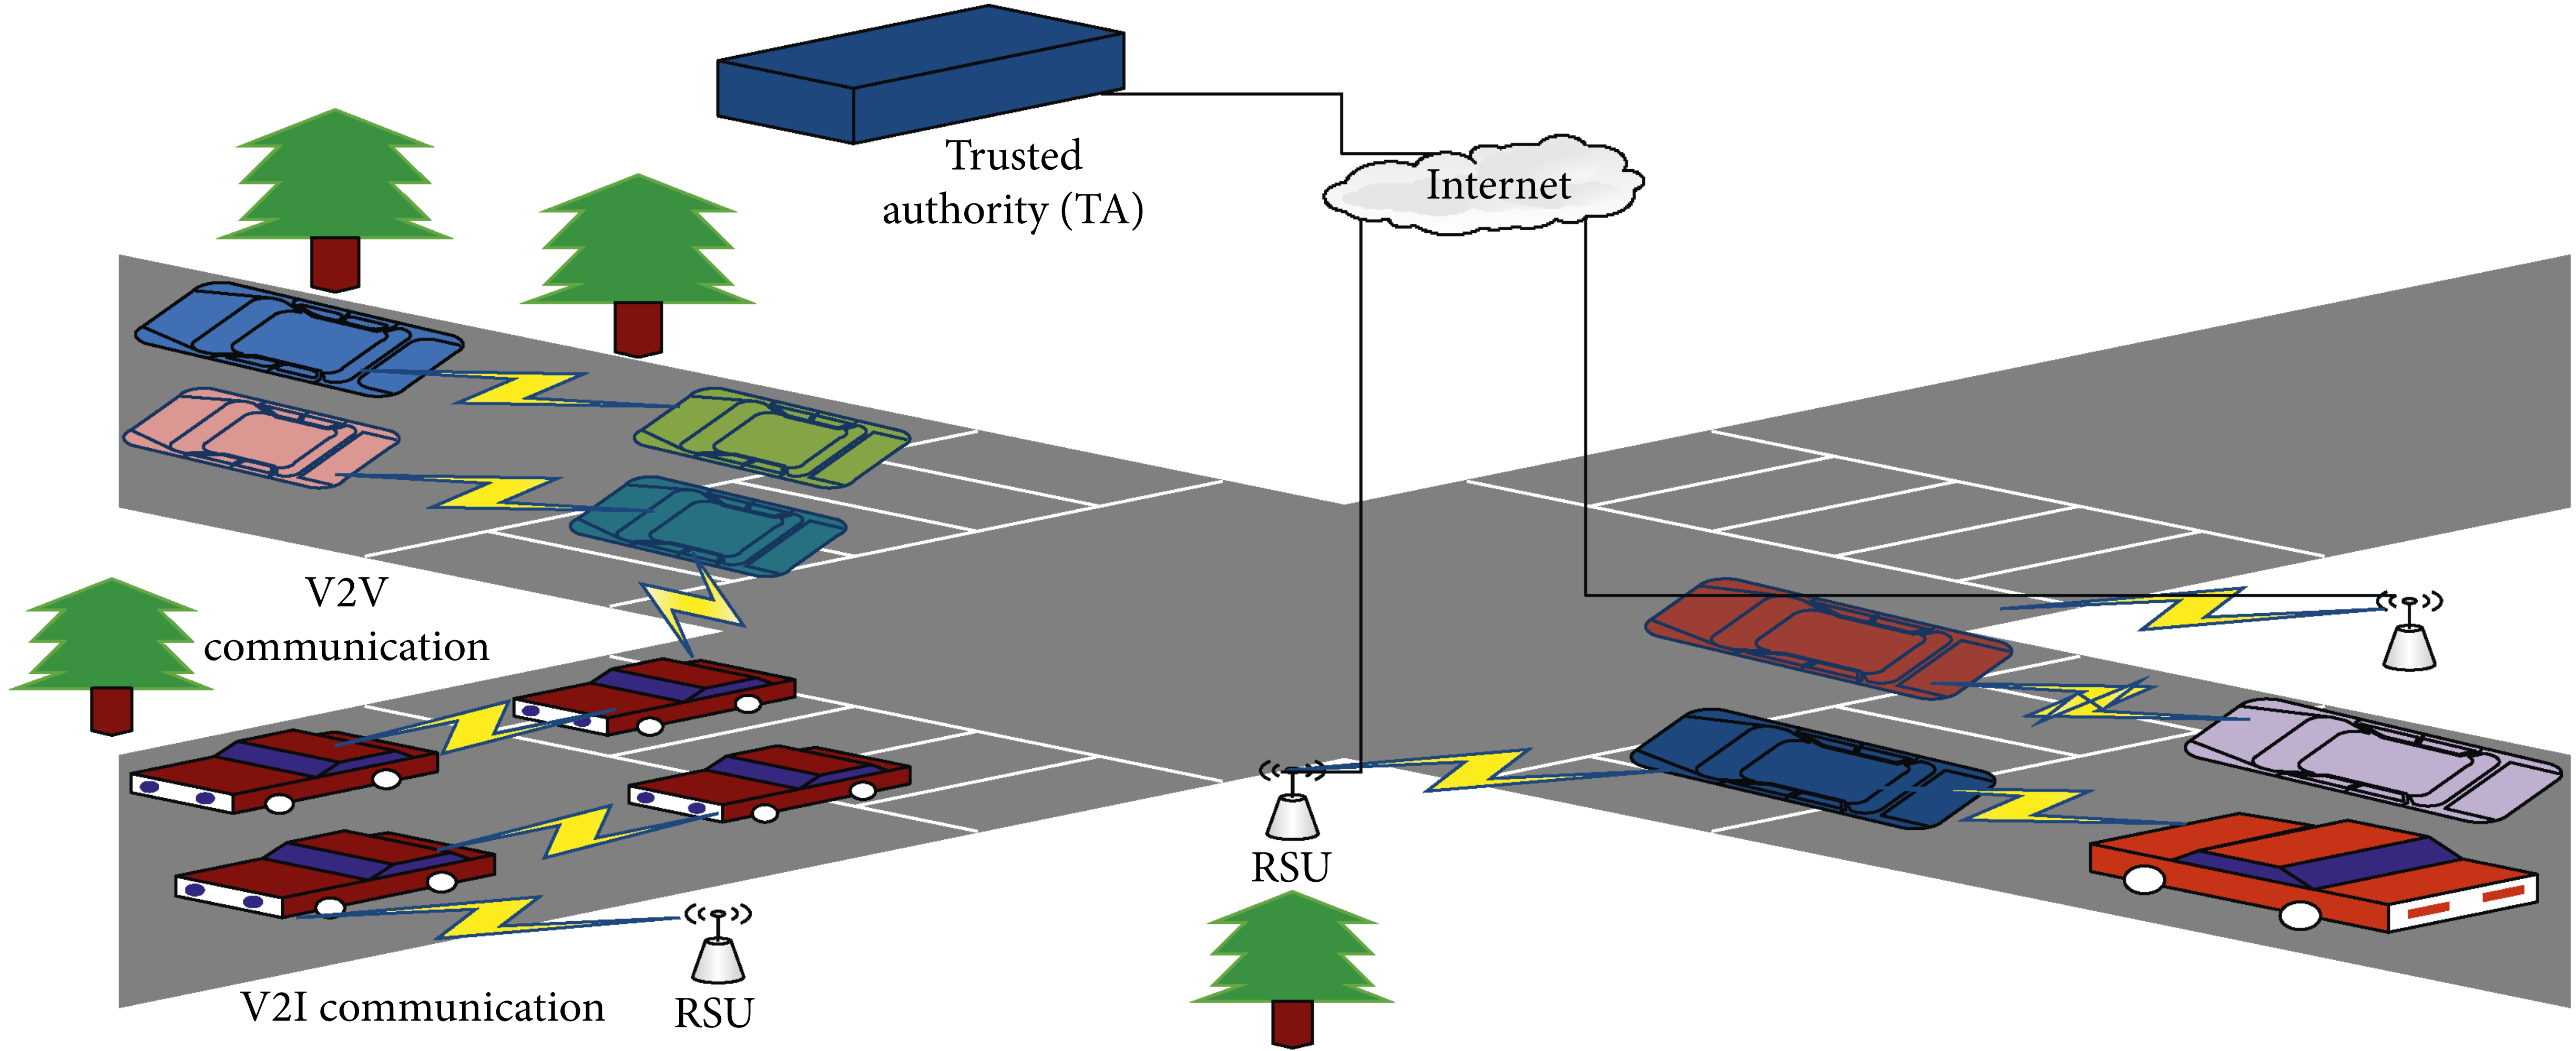
\includegraphics[width=0.8\textwidth]{img/vanetarchi.png}
\end{center}
  \caption{VANETs architectures ~\cite{vanet2}}
  \centering  
\label{VANETs architectures}
\end{figure}


Components of VANET are onboard units and roadside units as shown in Figure \ref{Vanets-Best-c}, we can see how communication is transmitted from the roadside unit to the onboard unit in the vehicle, and also a vehicle to vehicle communication. This creates a better share of information between vehicles.
VANET, vehicles act as nodes, unlike MANET that vehicles are set to move on a predefined road. The vehicles must follow traffic signs and signals and their velocity relies on the speed sign ~\cite{vanet2}. Wireless devices such
as; Personal Digital Assistant (PDA), Remote Keyless Entry Device, Mobile Phones, Laptops etc. are supported by VANET inside the vehicle. Due to the increase of mobile wireless devices, the demand for the vehicle-to-vehicle (V2V), vehicle-to-roadside (VRC), and vehicle-to-infrastructure (V2I) communication will
grow rapidly [20]. There are two type of communication infrastructure available by the VANET; first is the wireless ad hoc network, where there’s communication between vehicles without infrastructural support. Secondly, the communication between the vehicle and the road side unit. The IEEE defined standard of establishing a VANET is 802.11 or 802.16 (WIMAX) ~\cite{vanetusarlater}.


\begin{figure}[H]
\begin{center}
  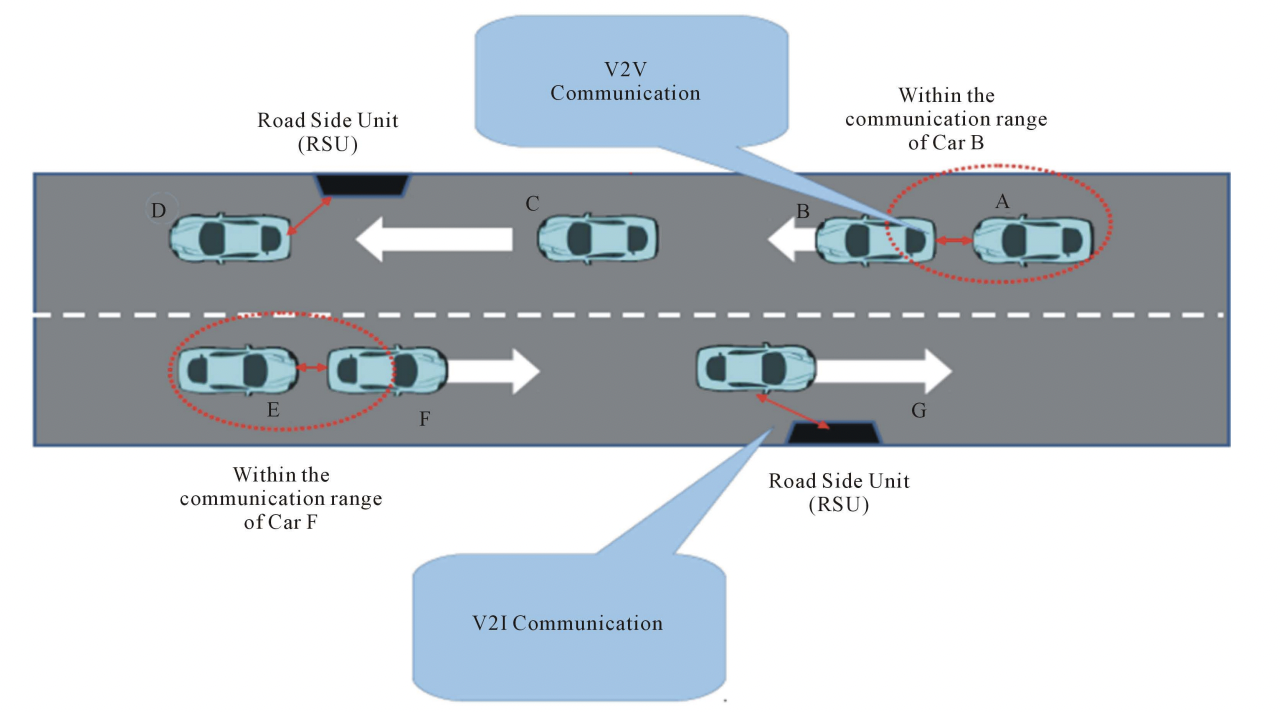
\includegraphics[width=0.9\textwidth]{img/v3.png}
\end{center}
  \caption{Typical components of VANET. ~\cite{vanetusarlater}}
  \centering  
\label{Vanets-Best-c}
\end{figure}



Therefore, it acts as a communication frontier between OBU and TA. RSUs can be placed at key indicators after a particular interlude to provide reliable network coverage and systematic operation. Therefore, the distance between nearby roadside units is kept within the range of each sequential RSU. OBU is fixed in the automobile and works as a central point for receiving, processing, and managing all data developed in the vehicle. It also serves as a source for exchanging data with the OBU of close-by vehicles as well as the RSU. TA is basically the foundation of the whole ITS and is usually connected to the RSU via fiber optic cable or wireless media. It manages the trust and safety of VANETs. TA verifies the entire network components via RSU and identifies the OBU that sends malicious packets and cancels the target node. TAs is in the center of the town and is managed by governments. The VANET system model is briefly described in Figure \ref{VANETs architectures} below.


\subsubsection{Definition of Terminology}
This list includes definitions related to the VANET protocol stacks and communication standards,  as well as some more generic 802.11 terms and definitions.

\begin{itemize}
    \item 

    OBU: In the context of VANET is the mobile communication device mounted on vehicles and equipped with one or more wireless interfaces, e.g., IEEE 802.11p, PC5, or Uu interfaces.
     \item 
    
    RSU: This is used to refer to the fixed communication devices deployed along the road to provide connectivity to vehicles. RSUs can be equipped with multiple wireless interfaces, e.g., IEEE 802.11p or PC5 interfaces. The RSU acts as a vehicular network infrastructure for communications using the specific wireless technologies and standards for vehicular communications.
     \item 
    WiFi AP: An AP that is compliant with the traditional IEEE Std 802.11 standard. We use the term traditional to refer, in an informal way, to the version of the 802.11 standard typically found in home and enterprise networks. However, we refer explicitly to the 11p amendment when we wish to refer to the 802.11 version specifically tailored for vehicular communications.
     \item 
    Base Station (BS): Generic term used to refer to the cellular network infrastructure. A BS can support 3G, 4th Generation of Broadband Cellular Networks (4G), or 5G technologies. In this survey, we use the term BS to refer to both eNB (4G) and gNB (5G).
     \item 
    IEEE 802.11p interface: A wireless interface fully compliant with the IEEE 802.11p amendment for vehicular communications. Both RSUs and OBUs can be equipped with interfaces supporting this standard.
     \item 
    ITS-G5 interface: A wireless interface fully compliant with the ITS-G5 specifications. Both RSUs and OBUs can be equipped with this interface.
     \item 
    PC5 interface: A wireless interface fully compliant with the 3rd Generation Partnership Project (3GPP) Release 14 specification for Cellular Vehicular To Everything (C-V2X) communications. Both RSUs and OBUs can be equipped with this interface.
     \item 
    Uu interface: A wireless interface fully compliant with cellular communications, i.e., 3G, 4G or 5G. OBUs can be equipped with these interfaces.

\end{itemize}



\subsection{Characteristics of VANETs}
VANETs is a dynamic ad hoc network that enables the vehicles converse with one another using fixed and mobile nodes offering numerous services, however with narrow access to the network’s infrastructure. Compared to the MANETs, the VANETs have high mobility features and normally vary in topology. In VANETs, vehicles or nodes move arbitrarily in the network, and their movement transforms the network topology. VANETs topology is complex and dynamic because of the strong mobility factor of nodes . The features of VANETs are mentioned below.

\subsubsection{}{High Mobility}

Because of the high mobility, the VANETs have good versatility relative to MANETs, and they play a significant role in modelling VANETs protocol. In VANETs, every node moves quickly; thus, vehicles’ mobility minimizes the communication time in the network ~\cite{vanet2} ~\cite{vanet2}].

\subsubsection{Driver Protection}

The VANETs might get better driver protection, improve traveller console, and support a better flow of traffic. The core benefit of VANETs is that nodes communicate straight to everyone ~\cite{vanet2}.

\subsubsection{Vibrant Network Topology}
In VANETs, the topology design is vibrant because the vehicle speed of mobility is very high. Therefore, the forecast of node position is very tough to compute. The high speed of vehicle networks is extra weak to attacks, and it is incredibly complicated to identify intruders and vehicles if something is wrong in a network ~\cite{vanet2}.

\subsubsection{Variable Network Density}
Due to high-speed mobility vehicles, traffic congestion or even lousy weather, the network may experience frequent or intermittent disconnection among nodes. In this situation, the nodes may receive proper guidance from the V2I infrastructure ~\cite{vanet2}.

\subsubsection{The Medium of Transmission}

Due to open wireless nature, these kinds of networks inherit all security vulnerabilities as posed to other traditional wireless networks ~\cite{vanets}.

\subsubsection{No Power Limits}

In MANETs, power is a grave problem; however, in VANETs the power is not a big problem since the OBU in vehicular entities bear sufficient battery and power resources necessary to carry out its communicative tasks ~\cite{vanet3},~\cite{vanet2}].

\subsubsection{Restriction of Transmission Power}
Wireless Access to Vehicle Environment (WAVE) limits the transmission power, which varies from 0 to 28.8°dBm with the corresponding coverage distance ranging from 10°m to 1km. Thus, the narrow power transfer may change the distance from the VANETS coverage ~\cite{vanet2}.


\subsubsection{Network Strength}
The signal strength of the network in VANETs depends on the traffic congestion, since it might gain more strength if there is no congestion or less traffic on the road. On the other hand, in case of traffic jams the signal quality might experience degradations ~\cite{vanet2}.

\subsubsection{Extensive Scale Network}
In VANETs, the network is highly scalable, since such kind of networks may experience highways, downtown areas, point of entries, and exit in the cities; hence, a massive number of nodes can be dynamically added or adjusted into the system ~\cite{vanet3}, ~\cite{vanetusarlater}.

\subsubsection{Extensive Computational Processing}

In VANETs, a large number of resources such as processors, colossal memory GPS, and antenna are embedded in vehicles. Such resources may require a massive computational capabilities and guidance to provide enhanced and trustworthy wireless communication for getting accurate information, i.e., live location, speed, and route of the vehicle ~\cite{vanetusarlater},~\cite{vanet2}. \par

VANET is a promising research area and for vehicular users. However, there are still several challenges to be faced, such as from a security perspective, integration with other emerging technology such as SDN, etc. VANET aims to reduce accidents on our roads and increase the flow of information between vehicles and road users.




\section{Software-Defined Vehicular Networks}
\label{Software-Defined Vehicular Networks}

The SDN paradigm is widely accepted as an encouraging way to revamp vehicular networks. SDN emerged as a stable approach to governing the network in an organized fashion. The flexibility of SDN makes it an attractive prospect for meeting the requirements of VANET scenarios. The centralized control, flexibility, and programming that are lacking in today's ad hoc wireless networks can be leveraged by applying SDN principles to VANETs. SDN concepts in VANET will simplify network management and also introduce new V2V and V2I services. It provides wireless resource optimization such as channel allocation, interference avoidance, packet routing in multi-hop multi path scenarios, efficient mobility, and network heterogeneity management. Being just a lightweight concept rather than a rigid framework (architecture), SDN integration into VANET is a considerable solution. Thus, the renewed architecture of VANET with SDN will reduce the impact of disconnection caused by vehicle mobility and increase communication reliability in VANETs, promoting the development of smart mobility. Following are the three main aspects of VANET integrated SDN:\par

\begin{itemize}
    \item Appropriate path:Extending SDN into VANET provides freedom of taking more detailed routing decisions. Sometimes, data traffic can be congested or excavated in VANET scenarios. It happens when all the nodes try to use the shortest path which will make some node very congested. When the controller detects scenarios mentioned above, then it can stop the currently executing process and start it again to increase utilization of the network and decreases the network blockages.
    \item Channel/frequency: Integrating SDN in VANET made available various accessible wireless interfaces or configurable radios (eg, cognitive radios). For instance, the controller will decide dynamically about the radio interface. It enables adaptive radio frequency selection for different sorts of traffic at the run time. The major aim of this is to conserve the frequency or channel for emergency services.
    \item Transmission power: It is an essential aspect for VANET to choose the proper energy level of wireless interfaces and its transmission range. In the VANET scenario, the controller collects the neighbor information from vehicles(wireless nodes). From this gathered information, it can be known when roads are empty or vehicles are farther away from each other. The controller adaptively assists every node to tune the power their level for the efficient packet delivery.
\end{itemize}


Through many state-of-the-art functionalities such as network function virtualization, centralized controls, and so on,the convergence of SDN and VANET emerges to provide a pleasing solution to implement the smart VANET, which is widely adopted as SDVN. Figure \ref{sdvn} shows generic architecture for SDVNs, which is compatible with both V2I and V2V.Vehicles are connected under a particular RSU, and all the RSUs are Open Flow-enabled. These RSUs are equipped with short range radio transceivers and can communicate with the available central global controller through cellular base stations. An application plane is connected with the global controller via the northbound API.Traditional networks are application-aware as they are tightly coupled systems and work as single integrated systems.But, SDVN systems generally have three logical groups of components, namely, infrastructure plane, control plane, and application plane. Figure \ref{sdvnV} shows the components involved in the software-defined vehicular network with some significant functions implemented in it. The SDVN functioning follows both the bottom-up and top-down paradigm. The vehicular information flows from bottom to up, whereas aggregated decisions and instructions propagated from top to down. In a software-defined vehicular network, the application layer is considered as a boss, whereas the control layer and infrastructure layer are supposed to be a brain and a body, respectively. The following subsection describes the component view of three-layered SDVN architecture ~\cite{Bhatia2019sdvn}.


\begin{figure}[H]
\begin{center}
  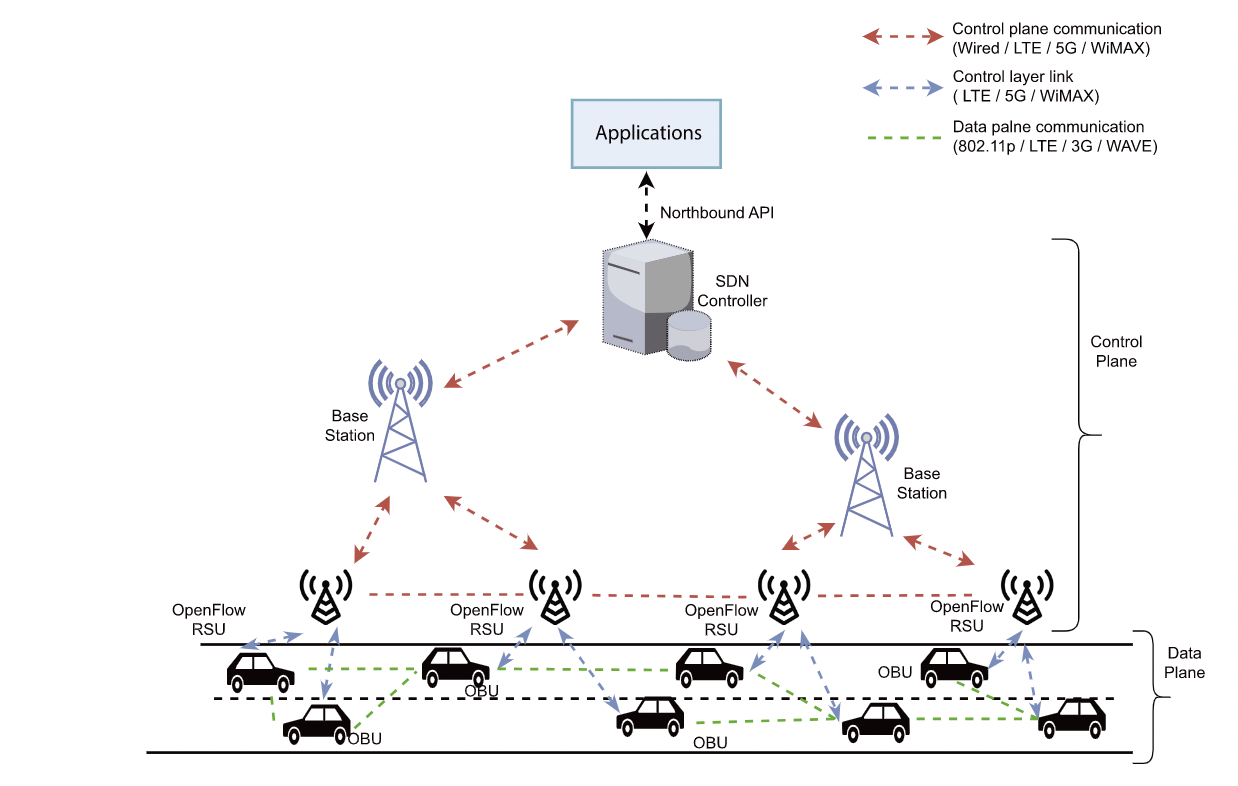
\includegraphics[width=0.9\textwidth]{img/sdvn1.png}
\end{center}
  \caption{Software-defined vehicular network (SDVN) architecture ~\cite{Bhatia2019sdvn}}
  \centering  
\label{sdvn}
\end{figure}


\subsection{Component view of SDVN}
\label{Component-view-of-SDVN}

This subsection aims to discuss the different possible components contained in each layer with their respective functionality in order to explore the full benefits of SDVN.

Infrastructure plan: The infrastructure plan comprises physical infrastructures and the devices that make up the network. It includes the various types of network devices such as mobile vehicles, OBUs and RSUs that are responsible for generating vehicular information such as routes, speed, positions, etc. It also comprises several forwarding devices such as routers,switches, etc. The heterogeneity of current vehicular networks is eliminated by introducing the overlay network in the infrastructure plane. The SDN switches provide the abstraction of all the vehicles and RSUs.\par
SDN Wireless Node: Refers to the mobile network device on the data plane known as vehicle or OBU that receives control messages from the SDN controller via RSU or cellular base station and is also responsible for collecting the various data from the network.



\begin{figure}[H]
\begin{center}
  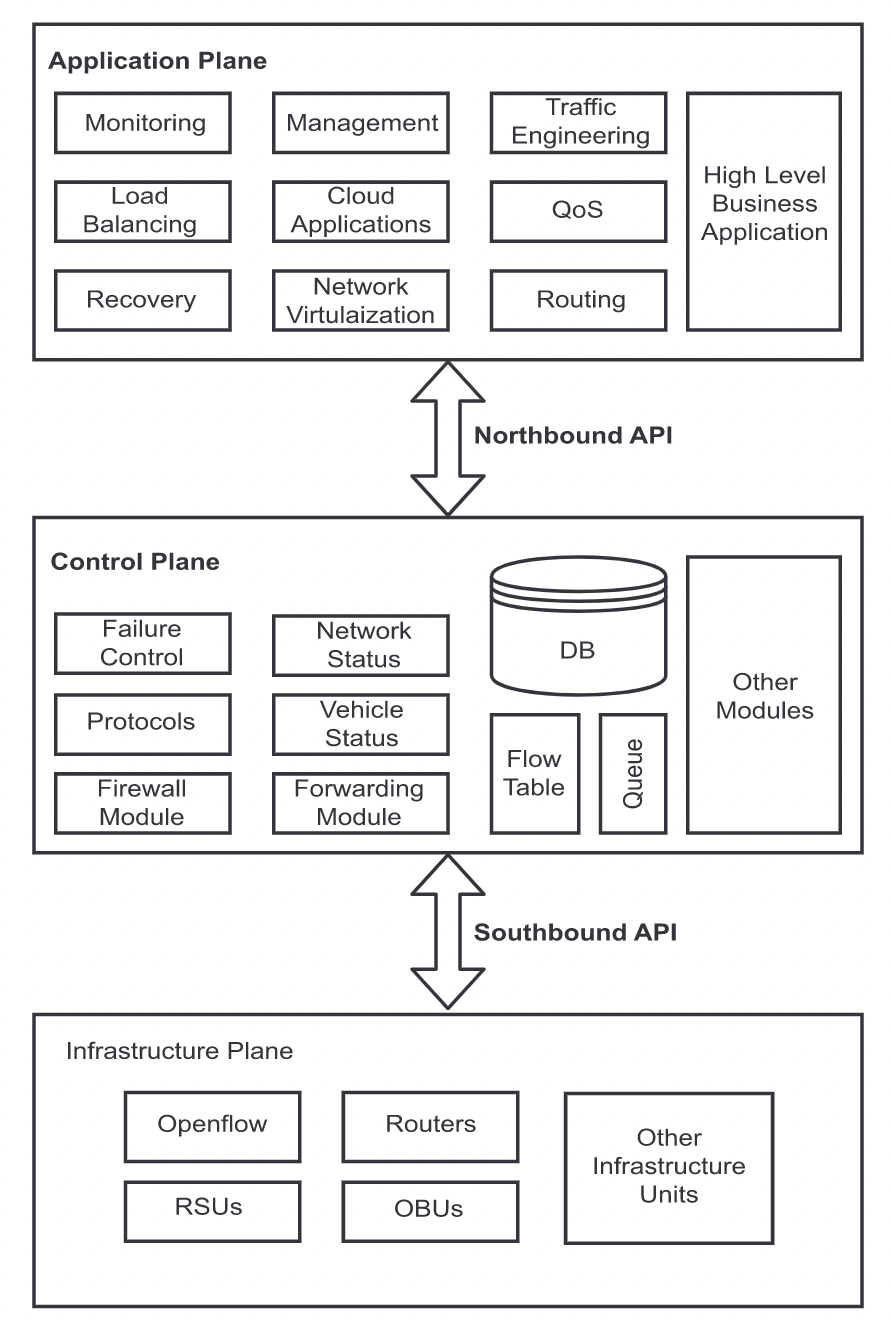
\includegraphics[width=0.6\textwidth]{img/sdvn2.png}
\end{center}
  \caption{Component diagram for software-defined vehicular network (SDVN) ~\cite{Bhatia2019sdvn}}
  \centering  
\label{sdvnV}
\end{figure}

SDN RSU:These are the stationary network devices on the edge of the data layer deployed along the road segments or with the cellular base station. Mostly, RSUs are open flow–enabled and its communication interface is compatible with wired, wireless, and LTE standards.\par

Cellular Base Station (BS):These are stationery network devices on the edge of the control layer. The cellular base station also termed as BS or Node B or eNode B. They work under the control of the SDN controller, and BS facilitates wireless connectivity between SDN controller and RSUs or OBUs using wireless communication technologies, ie, 3G, 4GLTE, Wi-Fi, WiMAX, 5G, CDMA.\par
Two types of approaches are favoured to make infrastructure plane layer adequate for sending and retrieving the data ~\cite{Bhatia2019sdvn}.
\begin{itemize}
    \item Vehicle-to-infrastructure (V2I):Under this vehicular communication environment, vehicles can communicate with deployed RSUs and are not concerned with the information of other vehicles. As all the devices along the path to vehicles are static, also known as fixed infrastructure plane.
    \item Vehicle-to-vehicle (V2V):This approach is suitable when all the traditional mobile vehicles are equipped with the special on-board units that support SDN functionalities (also called a mobile infrastructure plane). In V2V approach, each SDN-compatible vehicle monitors the vehicle attributes, ie, id, speed, direction, etc. The concept of clustering is introduced in this approach. This information is periodically forwarded to the cluster head. The cluster head isone of the vehicle playing the role of local controller and maintains the flow table.\par
\end{itemize}


Control plane: It acts as a core part of software-defined VANET consisting of SDN controller and other modules such as firewall module, failure control, protocols, system status, database, flow tables, etc. It takes care of centralization by providing the global view of the entire network.\par
SDN controller:SDN controller is a logical entity that collects information from infrastructure plane as per the requirement of the application plane. It leverages the architecture with storage and calculation capabilities. The controller also provides an abstract view of the network including statistics and events.\par
The control plane also has two types that are fixed control plane and mobile control plane.\par

\begin{itemize}
    \item Fixed control plane:It has all the controllers fixed on the infrastructure. The global controller (GC) is set at one place or in the cloud server. Local controllers are configured on RSUs or cellular base stations and are used to collect and filter out the received data. All controllers have several interfaces for communicating up and down.
    \item Mobile control plane:It has its global controller located at the central unit or in the cloud. The local controllers(LC) are deployed in the mobile vehicle itself. Tasks are divided between GC and LCs. The global controllers respond to requests that require complex and powerful computing resources. It also serves the bandwidth sensitive demands or asks for the global view of the network. The LCs take care of the normal running requests and become active only when that vehicle is chosen as the cluster head. LC comes with limited memory and computational power, so it acts as a slave of the global controllers.
\end{itemize}\par

 Application plane:This plane consists of various applications that communicate with control layer plane and provides insights of the network by fetching the information from the SDN controller. There are the plethora of applications that can be executed such as monitoring, QoS, analytics, recovery, security, routing, load balancing, network virtualization and management, traffic engineering, cloud computing, or business applications used. The prediction model can be trained, which predicts the location of vehicles based on historical information. Another example is an analytic application that can be incorporated to recognize suspicious network activity. Application layer provides an open interface for optimizing network function.\par
 The advantages of integrating SDN into VANETs are due to the decoupling of the three layers which are mentioned above. APIs such as northbound, southbound, eastbound and westbound are implemented to connect this decoupled layers with each other. The northbound API is implemented between the controller (control plane) and applications(application plane), while the southbound API is implemented between the controller and the physical networking hardware (data plane layer or infrastructure plane) ~\cite{Bhatia2019sdvn}.


\subsection{Architectural modes and access technologies}
\label{Architectural-modes-and-access-technologies}


The previous subsection (\ref{Component-view-of-SDVN}) highlighted the architecture and components of SDVN where almost all SDVN comprises three planes. Existing SDVNs do not differ in these plans, but vary depending on how these plans are implemented in real-life scenarios, the protocol suite, and the architectural strategies of the SDVN. We will now look at existing SDVNs based on key attributes according to the taxonomy mentioned in Figure \ref{sdvnVv}.\par

\begin{figure}[H]
\begin{center}
  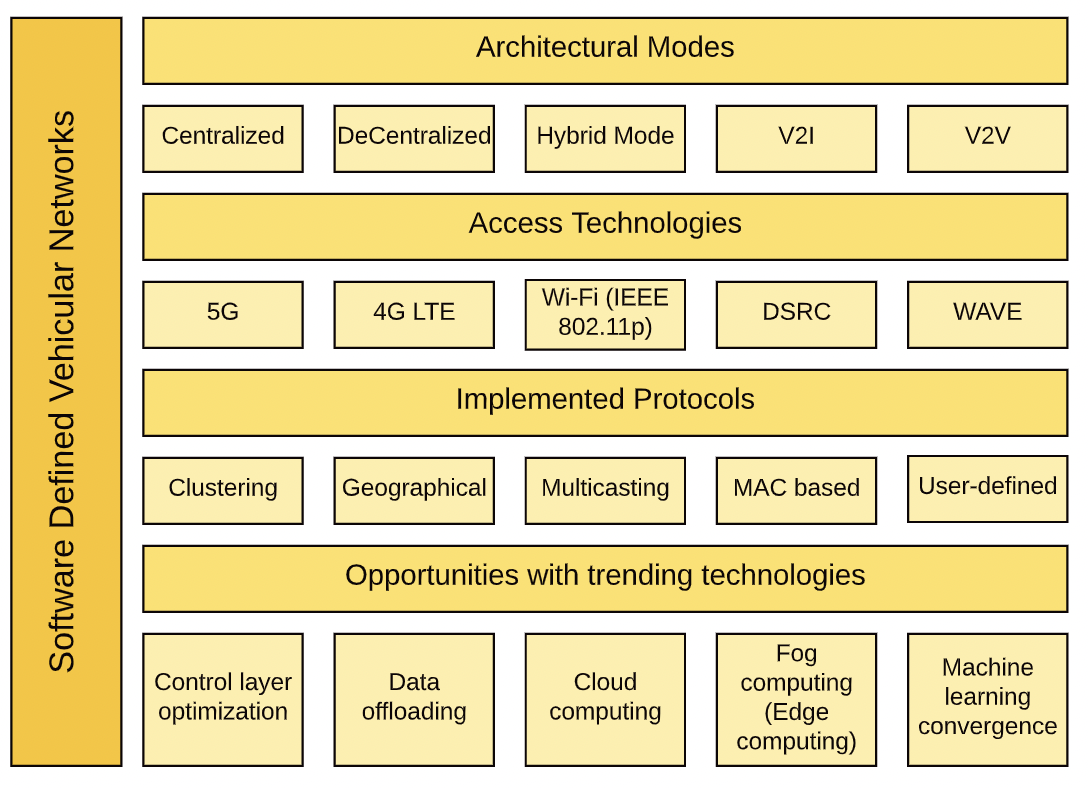
\includegraphics[width=0.6\textwidth]{img/taxonomias sdvn.png}
\end{center}
  \caption{Taxonomy of software-defined vehicular network (SDVN) ~\cite{Bhatia2019sdvn}}
  \centering  
\label{sdvnVv}
\end{figure}

 Over half-decade, there are lots of tools and technologies used by researchers to implement the SDN concepts along with VANET system. Many researchers in previous studies50–53have shown their efforts to implement SDN capabilities into VANET using various technologies such as SUMO, OMNET++, VEINS, Mininet-WiFi, Network simulator 3, Floodlight, ONOS, POX61controller, etc. Fontes et al have used Mininet modules for node car architecture, OpenFlow-enabled controller is implemented to manage cars, RSUs, and eNodeBS. The node cars have root spine switch installed for LTE and Wi-Fi communication. Here, node car captures a short duration video for safety purpose, video surveillance, or traffic analysis is done using the on board camera. Then, the SDN controller chose proper routing path and communication technology for that captured video to send over the central repository. Berk et al52uses a Raspberry Pi module as an OpenFlow-enabled RSU. The open daylight SDN controller is connected with all the RSUs through wired LAN. Furthermore, RSUs are connected with wireless internet access points (AP) through Wi-Fi. Here, instead of cars, smartphones are considered as mobility nodes. The smartphone connects to the wireless internet with which RSUs are linked ~\cite{Bhatia2019sdvn}.\par
 
\section{Selected tools}
\label{tools}

To achieve the objectives outlined (section \ref{objectives}), some essential tools were defined, we will discuss about these tools in the following subsections.
Based in our objectives we should be fulfilled same requiremnt

\subsection{SUMO - Simulation of Urban MObility}
\label{SUMO}

SUMO is abbreviated as Simulation of Urban Mobility ~\cite{dlr127994}. 

This simulator assumes a critical role in facilitating network imports and demand modeling functionalities, making it indispensable for various research projects.

One of the distinguishing features of SUMO is its flexibility in accommodating custom models. Moreover, it offers a plethora of application programming interfaces (APIs) that enable remote control of the simulation process. This capability allows researchers to fine-tune and optimize their experiments, thereby enhancing the overall simulation experience.

Over the years, SUMO has been leveraged within numerous projects aimed at addressing diverse research inquiries. For instance, investigations into vehicle route choice have been conducted, encompassing the development and evaluation of novel methodologies. Notably, the evaluation of eco-aware routing strategies based on pollutant emission as well as explorations of network-wide impacts of autonomous route selection have been carried out using SUMO.

The versatility of SUMO extends beyond conventional research domains. Notably, the software has been employed to provide traffic forecasts for local authorities during significant events such as the Pope's visit to the City of Cologne in 2005 and the Soccer World Cup in 2006. Additionally, SUMO has been instrumental in facilitating simulated in-vehicle telephony behavior, enabling the evaluation of GSM-based traffic surveillance systems.

Furthermore, SUMO has gained significant popularity within the Vehicle-to-Everything (V2X) community. Its capabilities in generating realistic vehicle traces and evaluating applications in conjunction with network simulators have made it an indispensable tool for V2X researchers seeking real-world validation and performance assessment.

In summary, SUMO stands as a versatile and widely embraced software tool, enabling transportation researchers to tackle a diverse array of research questions with utmost precision and efficiency. 


The applications of SUMO in recent simulation endeavors encompass a broad spectrum of research topics, reflecting its versatility and relevance. 

\begin{figure}[H]
\begin{center}
  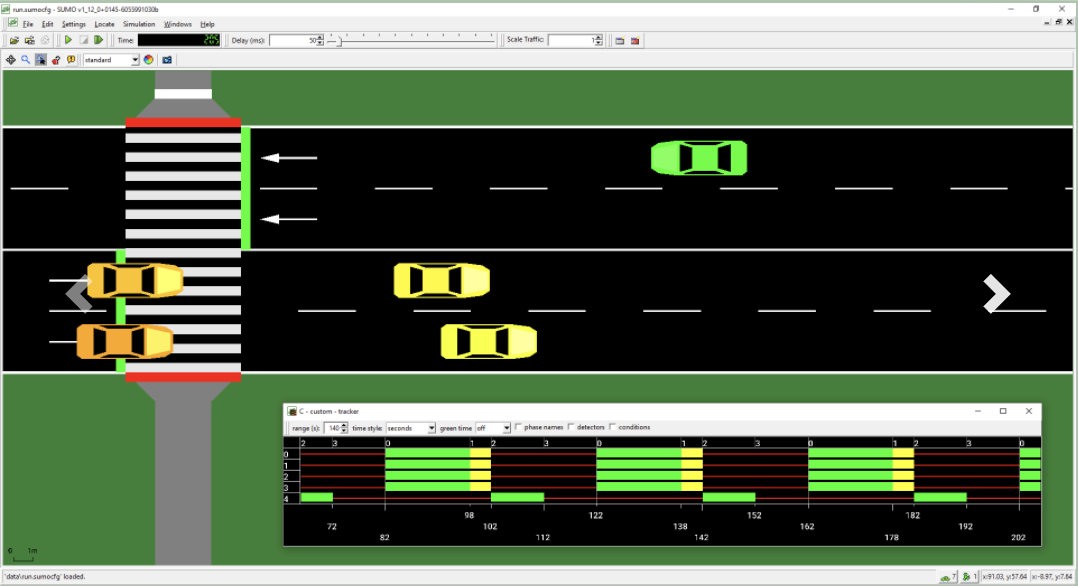
\includegraphics[width=0.6\textwidth]{img/sumo.png}
\end{center}
  \caption{SUMO simulator}
  \centering  
\label{sumo}
\end{figure}


\subsection{Mininet-Wifi}
\label{Mininet-Wifi}

Mininet-WiFi is a fork of the Mininet SDN network emulator and extended the functionality of Mininet by adding virtualized WiFi stations and access points based on the standard Linux wireless drivers and the 80211-hwsim wireless simulation driver. We added classes to support the addition of these wireless devices in a Mininet network scenario and to emulate the attributes of a mobile station such as position and movement relative to the access points.
The Mininet-WiFi extended the base Mininet code by adding or modifying classes and scripts. So, Mininet-WiFi adds new functionality and still supports all the normal SDN emulation capabilities of the standard Mininet network emulator.

Mininet-WiFi works fine on any Ubuntu distribution from 14.04 onwards, although there are some bugs in Ubuntu 16.04 ~\cite{mininet-wifibook}.

\subsection{Architecture and Components}

The main components that make part of the development of Mininet-WiFi are illustrated in Figure \ref{componentes-mini}. In the kernel-space the module mac80211-hwsim is responsible for creating virtual Wi-Fi interfaces, important for stations and access points. Continuing in the kernel-space, MLME (Media Access Control Sublayer Management Entity). is realized in the stations side, while in the user-space the hostapd is responsible for this task in the AP side.\par
Mininet-WiFi also uses a couple utilities such as iw, iwconfig e o wpa-supplicant. The first two are used for interface configuration and for getting information from wireless interfaces and the last one is used with Hostapd, in order to support WPA (Wi-Fi Protected Access), among other things. Besides them, another fundamental utility is TC (Traffic Control). The TC is an user-space utility program used to configure the Linux kernel packet scheduler, responsible for controlling the rate, delay, latency and loss, applying these attributes in virtual interfaces of stations and APs, representing with higher fidelity the behavior of the real world ~\cite{mininet-wifibook}.\par
Figure \ref{compomininet-conect} depicts the components and connections in a simple topology with two hosts created with Mininet-WiFi, where the newly implemented components (highlighted in gray) are presented along the original Mininet building blocks.\par
More specifically, we added WiFi interfaces on stations that now are able to connect to an access point through its (wlanX) interface that is bridged to an OpenFlow switch with AP capabilities represented by (ap1). Similar to Mininet, the virtual network is created by placing host processes in Linux OS network namespaces interconnected through virtual Ethernet (veth) pairs. The wireless interfaces to virtualize WiFi devices work on master mode for access points and managed mode for stations.\par

\textbf{Stations:} Are devices that connect to an access point through authentication and association. In our implementation, each station has one wireless card (staX-wlan0 - where X shall be replaced by the number of each station). Since the traditional Mininet hosts are connected to an access point, stations are able to communicate with those hosts.\par
\textbf{Access Points:} Are devices that manage associated stations. Virtualized through hostapd daemon and use virtual wireless interfaces for access point and authentication servers. While virtualized access points do not have (yet) APIs allowing users to configure several parameters in the same fashion of a real one, the current implementation covers the most important features, for example ssid, channel, mode, password, cryptography, etc ~\cite{mininet-wifibook}.\par
Both stations and access points use cfg80211 to communicate with the wireless device driver, a Linux 802.11 configuration API that provides communication between stations and mac80211. This framework in turn communicates directly with the WiFi device driver through a netlink socket (or more specifically nl80211) that is used to configure the cfg80211 device and for kernel-user-space communication as well.\par


\begin{figure}[H]
\begin{center}
  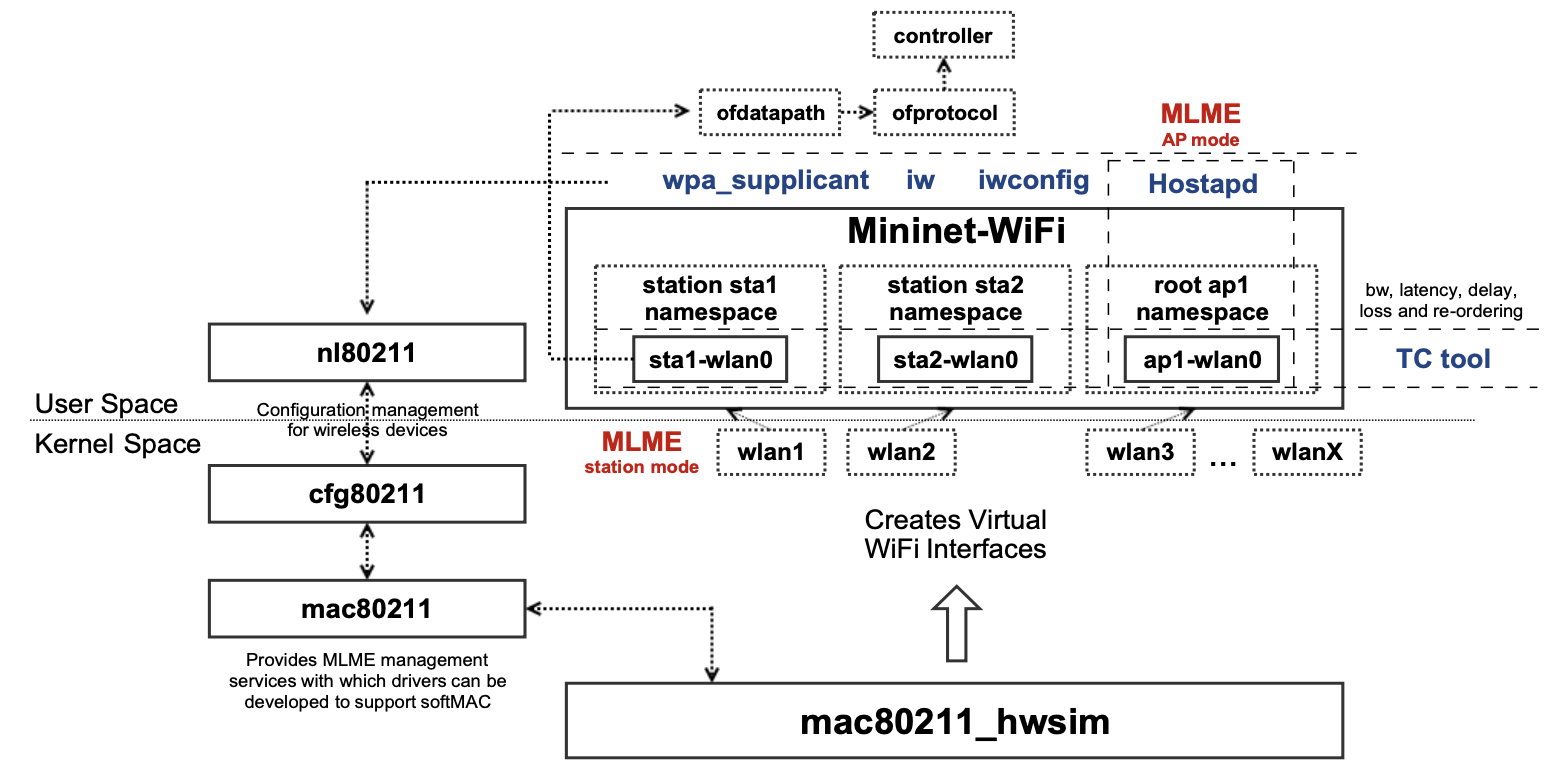
\includegraphics[width=0.5\textwidth]{img/12.png}
\end{center}
  \caption{Mininet-WiFi Components ~\cite{mininet-wifibook}}
  \centering  
  \label{componentes-mini}
  
\begin{center}  
  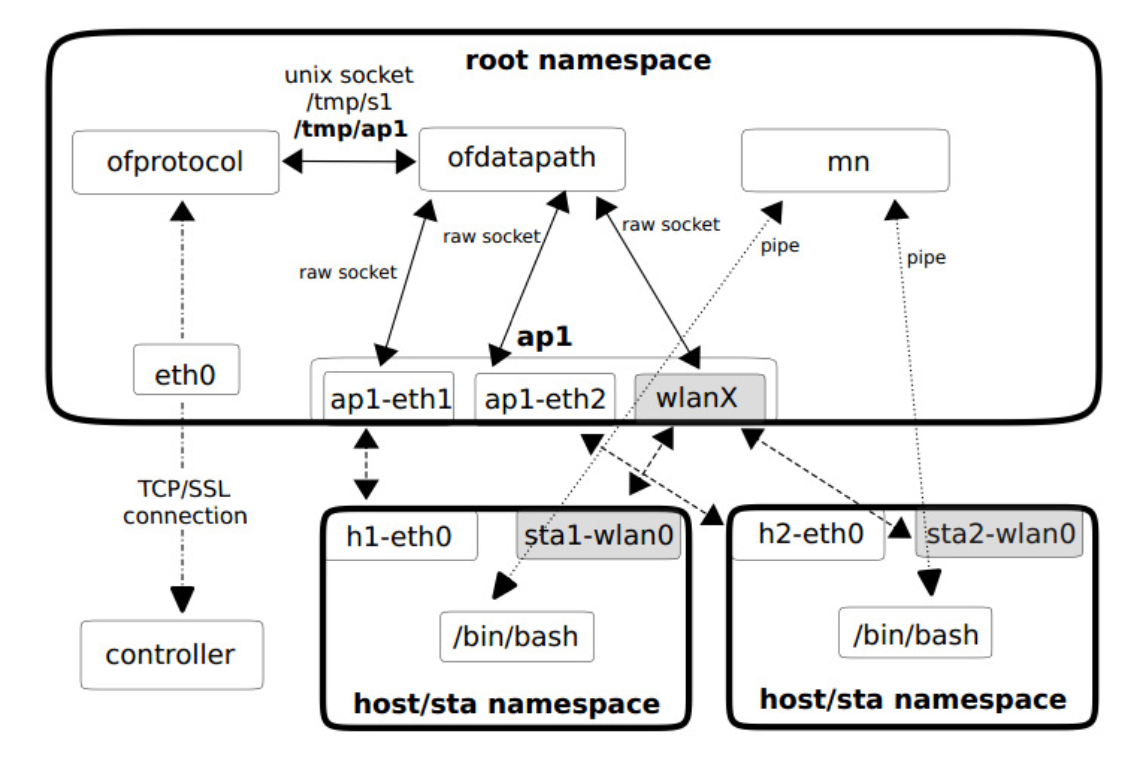
\includegraphics[width=0.5\textwidth]{img/13.png}
\end{center}
  \caption{Components and connections in a two-host network created with Mininet-WiFi ~\cite{mininet-wifibook}}
    \centering  
  \label{compomininet-conect}
\end{figure}

\subsection{Ryu Controller}
\label{Ryu-Controller}

Ryu is a component-based software-defined network controller. Ryu provides software components with a well-defined API that makes it easy for developers to create new network management and control applications. One of Ryu's advantages is the fact that it supports all versions of OpenFlow. It is a python controller and is based on modules, with a fixed base that aims to launch the controller and forward messages to the different registered modules, being these to take the actions on the package.\par
The framework facilitates development by providing the basic functions for controlling the data plane and the functions that are common to SDN applications. The functions that are features of Ryu are described in the following subsections.\par


\subsection{Philosophy}

\begin{itemize}
    \item  Agile
    Framework for SDN application development instead of all-purpose big monolithic ‘controller’.
    \item Flexible
    Vendor-defined “Northbound” APIs are not enough to differentiate.
\end{itemize}

\subsubsection{Component-based framework}

\begin{itemize}
    \item Your application consists of component(s)\par
        Ryu provides a bunch of components useful for SDN
applications (see figure \ref{Ryu-compo}).\par
        You can modify the existing components and implement your new components. \par
        Combines the components to build your application.\par
\end{itemize}

\subsection{Component implementation}

\begin{itemize}
    \item  Use favorite language \par
    Your component can work together with the existing components with Ryu’s ‘standard’ messaging way.\par
    You can run the existing software (such as routing protocol daemons) as Ryu component with some modification.\par
    \item Components included in Ryu \par
    
    Implemented in Python.\par
    A component consists of python thread(s) or OS process(s).\par
\end{itemize}

\begin{figure}[H]
\begin{center}
  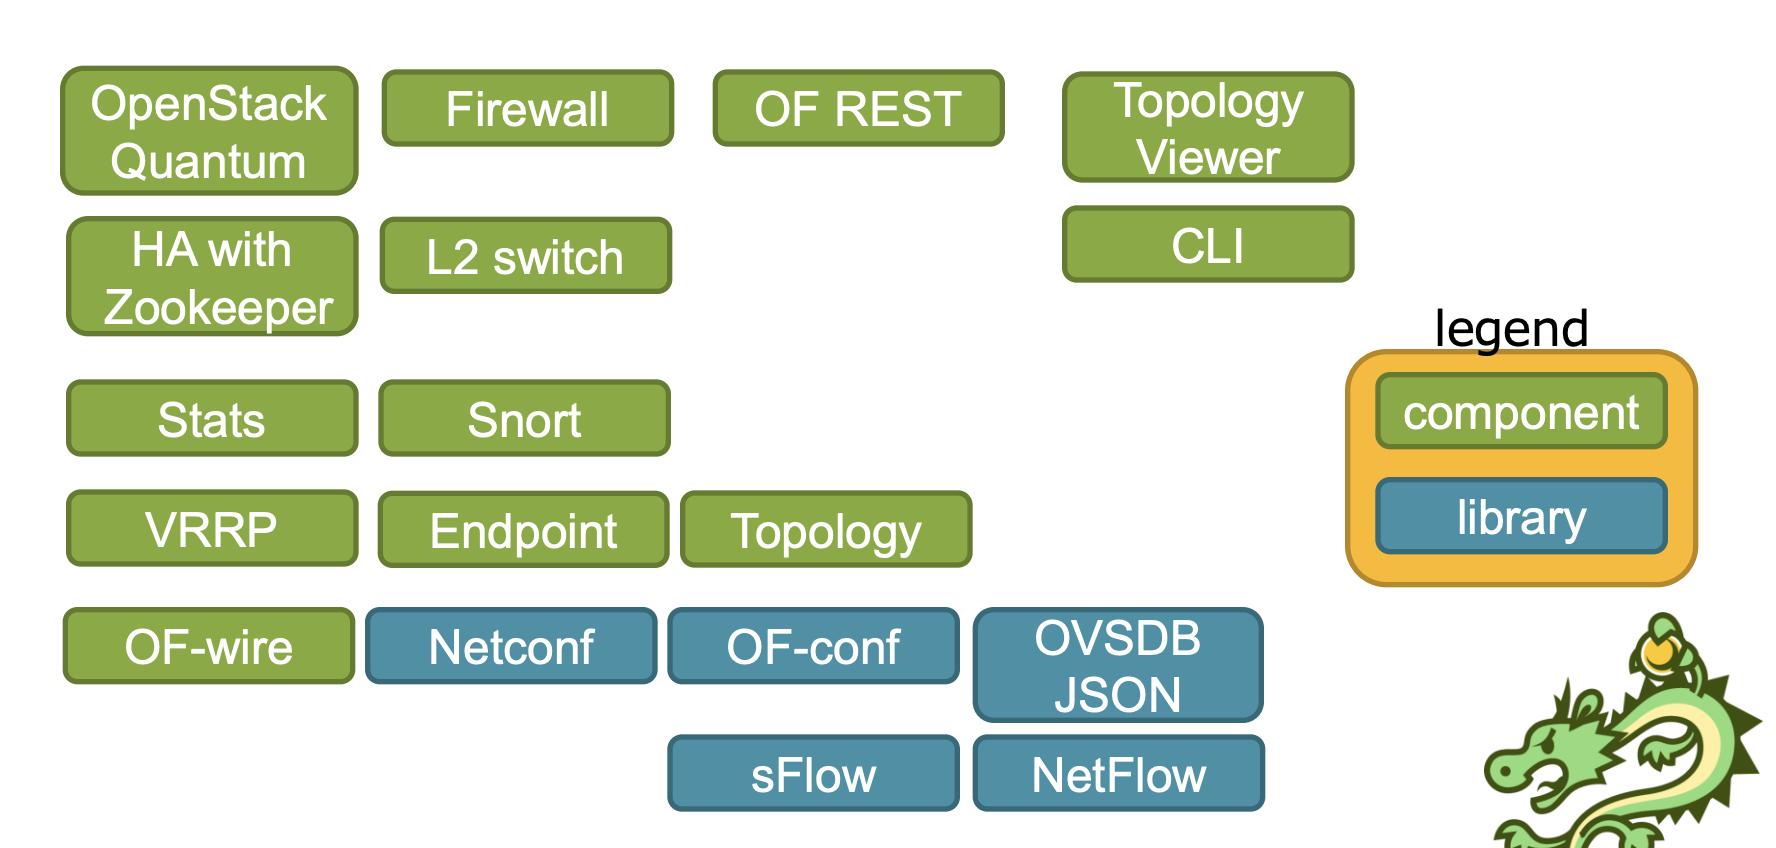
\includegraphics[width=0.8\textwidth]{img/Ryucompo.png}
\end{center}
  \caption{Components and libraries included in Ryu}\par
  From: https://ryu-sdn.org/slides/ONS2013-april-ryu-intro.pdf
  \centering  
\label{Ryu-compo}
\end{figure}


\section{Summary}

In this chapter, an overview was made of the various essential topics for the development of this work, from the basic principles of SDN, in which the layers that constitute the architecture of SDN are inserted. There was also an overview of Vanets, the basic principles of a Vanet and its leverage with the SDN. We also present the convergence of SDN and VANETs in detail. The components of the SDVN architecture were also analyzed, such as infrastructure plane, control plane and application plane of SDVN, architecture modes and access technologies. Finally, we present some tools that will be essential for the experiments that we have defined as a proposal for this thesis.




%As we can see on Figure \ref{Figure-Northbound}
%As we can see on subsesion\ref{section-SDN}






%\subsection{Optional}
%You may wish to use the \conexp{Concept-Explorer} tool.

\part{Core of the dissertation}% Here started the second part of project


%\chapter{The problem and its challenges}
         %The problem and its challenges.
\chapter{{Simulations}}
\section{Introduction}
\section{Results}


\section{Illustrative tests of solution operation}
%\section{Images}


\part{Conclusions}

\chapter{Contribution}
	%Main result(s) and their scientific evidence
\section{Introduction}
\section{Summary}

%\chapter{Applications}
%	Application of main result (examples and case studies)
%\section{Introduction}
%\section{Summary}

\chapter{Conclusions and future work}
	%Conclusions and future work.
\section{Conclusions}
\section{Future work}
		
\bookmarksetup{startatroot} % Ends last part.
\addtocontents{toc}{\bigskip} % Making the table of contents look good.
\cleardoublepage

%----------------- Bibliography (needs bibtex) --------------------------------%
\bibliography{dissertation}
%----------------- Index of terms (needs  makeindex) --------------------------%
\printindex
%------------------------------------------------------------------------------%
	
	\appendix
	\renewcommand\chaptername{Appendix}

	% Add appendix chapters

\part{Appendices}

\chapter{Support work}
	%Auxiliary results which are not main-stream

\chapter{Details of results}
         %Details of results whose length would compromise readability of main text.

\chapter{Listings}
	%Should this be the case

\chapter{Tooling}
	%(Should this be the case)

	%Anyone using \Latex\ should consider having a look at \TUG,
%	the \tug{\TeX\ Users Group}
	
\begin{backcover}
\thispagestyle{empty} \pagecolor{white} \textcolor{black} {\fontfamily{phv}\fontseries{mc}\selectfont ~\vfill
\noindent
%NB: place here information about funding, FCT project, etc in which the work is framed. Leave empty otherwise.
%
\vfill ~}
\end{backcover}

\end{document}

